%% 
%% Copyright 2007-2024 Elsevier Ltd
%% 
%% This file is part of the 'Elsarticle Bundle'.
%% ---------------------------------------------
%% 
\documentclass[preprint,12pt]{elsarticle}

%% Use the option review to obtain double line spacing
%% \documentclass[authoryear,preprint,review,12pt]{elsarticle}

%% Use the options 1p,twocolumn; 3p; 3p,twocolumn; 5p; or 5p,twocolumn
%% for a journal layout:
%% \documentclass[final,1p,times]{elsarticle}
%% \documentclass[final,1p,times,twocolumn]{elsarticle}
%% \documentclass[final,3p,times]{elsarticle}
%% \documentclass[final,3p,times,twocolumn]{elsarticle}
%% \documentclass[final,5p,times]{elsarticle}
%% \documentclass[final,5p,times,twocolumn]{elsarticle}

%% For including figures, graphicx.sty has been loaded in
%% elsarticle.cls. If you prefer to use the old commands
%% please give \usepackage{epsfig}


\usepackage{amssymb}
\usepackage{amsmath}
\usepackage{lineno}
\usepackage[colorinlistoftodos,prependcaption,textsize=tiny]{todonotes}
\journal{Journal of Computer Languages}

\begin{document}

\begin{frontmatter}

 \author{Shuai Fu}

 \author{Tim Dwyer}

 \author{Peter J. Stuckey}

 \author{John Grundy}


 \affiliation{organization={Monash University}, country={Australia}}


\title{GeckoGraph: A Visual Language for Polymorphic Types}

%% Abstract
\begin{abstract}
Polymorphic type is an important feature in most strongly typed programming languages. They allow functions to be written in a way that can be used with different data types, while still enforcing the relationship and constraints between the values. However, programmers often find polymorphic types difficult to use and understand, and tend to reason with a mindset of concrete types. We propose GeckoGraph, a graphical notation for types. GeckoGraph aims to complement traditional text-based type notation by making reading, understanding, and comparing types easier. We conducted a large-scale user study using GeckoGraph, comparing it to text-based type notation. To our knowledge, this is the largest controlled user study on functional programming ever conducted. 
The results show no overall significant differences in task completion time or success rate. However, we observed a modest improvement in success rate among beginner participants. For the most challenging task, GeckoGraph improved success rates by 14.5\% for beginners and 11.2\% for less experienced users. These findings suggest that GeckoGraph has potential as a teaching and learning aid for polymorphic type systems.
\end{abstract}

%% Keywords
\begin{keyword}
%% keywords here, in the form: keyword \sep keyword

%% PACS codes here, in the form: \PACS code \sep code

%% MSC codes here, in the form: \MSC code \sep code
%% or \MSC[2008] code \sep code (2000 is the default)
Polymorphic Types \sep Functional Programming \sep Visual Languages \sep Visualization
\end{keyword}

\end{frontmatter}

\linenumbers

\section{Introduction} \label{sec:intro}
In programming languages, a polymorphic type \cite{Cardelli1987-fp} can represent values of different types while providing an interface to describe common behaviors for those values. Polymorphic types are one of the oldest topics in programming language theory \cite{Cardelli1987-fp}. They are central to the succinctness of statically-typed languages, while also enabling a high degree of type-safe abstraction and reusability. Polymorphic types are available in many programming languages, from functional languages such as Haskell and ML to imperative and multi-paradigm languages such as Rust\cite{Klabnik_undated-wx} and Go\cite{Griesemer_undated-ff}.

% Polymorphism allows programs to be written in a way that is more generic and adaptable to different data types, enabling greater flexibility and code reuse. Polymorphic types are ideal for modeling abstractions, such as properties of mathematical objects and laws that hold on these objects. 

While promoting robustness and code reusability, polymorphic types present challenges in learning and comprehension, particularly for novice users \cite{Jun2000-ec, Jun2000-yu}; as it is often argued that the expressiveness power of type systems often comes at the cost of their usability~\cite{Hage2020-hg}. Research indicates that humans tend to focus on concrete types and rely on polymorphic type checking only as a last resort. Moreover, polymorphic types often complicate type error usability. During type checking, compilers frequently generate new polymorphic type variables temporarily. These variables are typically discarded after type checking unless a type error occurs, in which case they are referenced in error messages. Consequently, programmers often face the task of resolving type errors involving type variables they did not explicitly author (Fig. \ref{fig:example-foldable}). Unfortunately, not many studies focus on the \textit{usability} of polymorphic types. 

\begin{figure}[]
  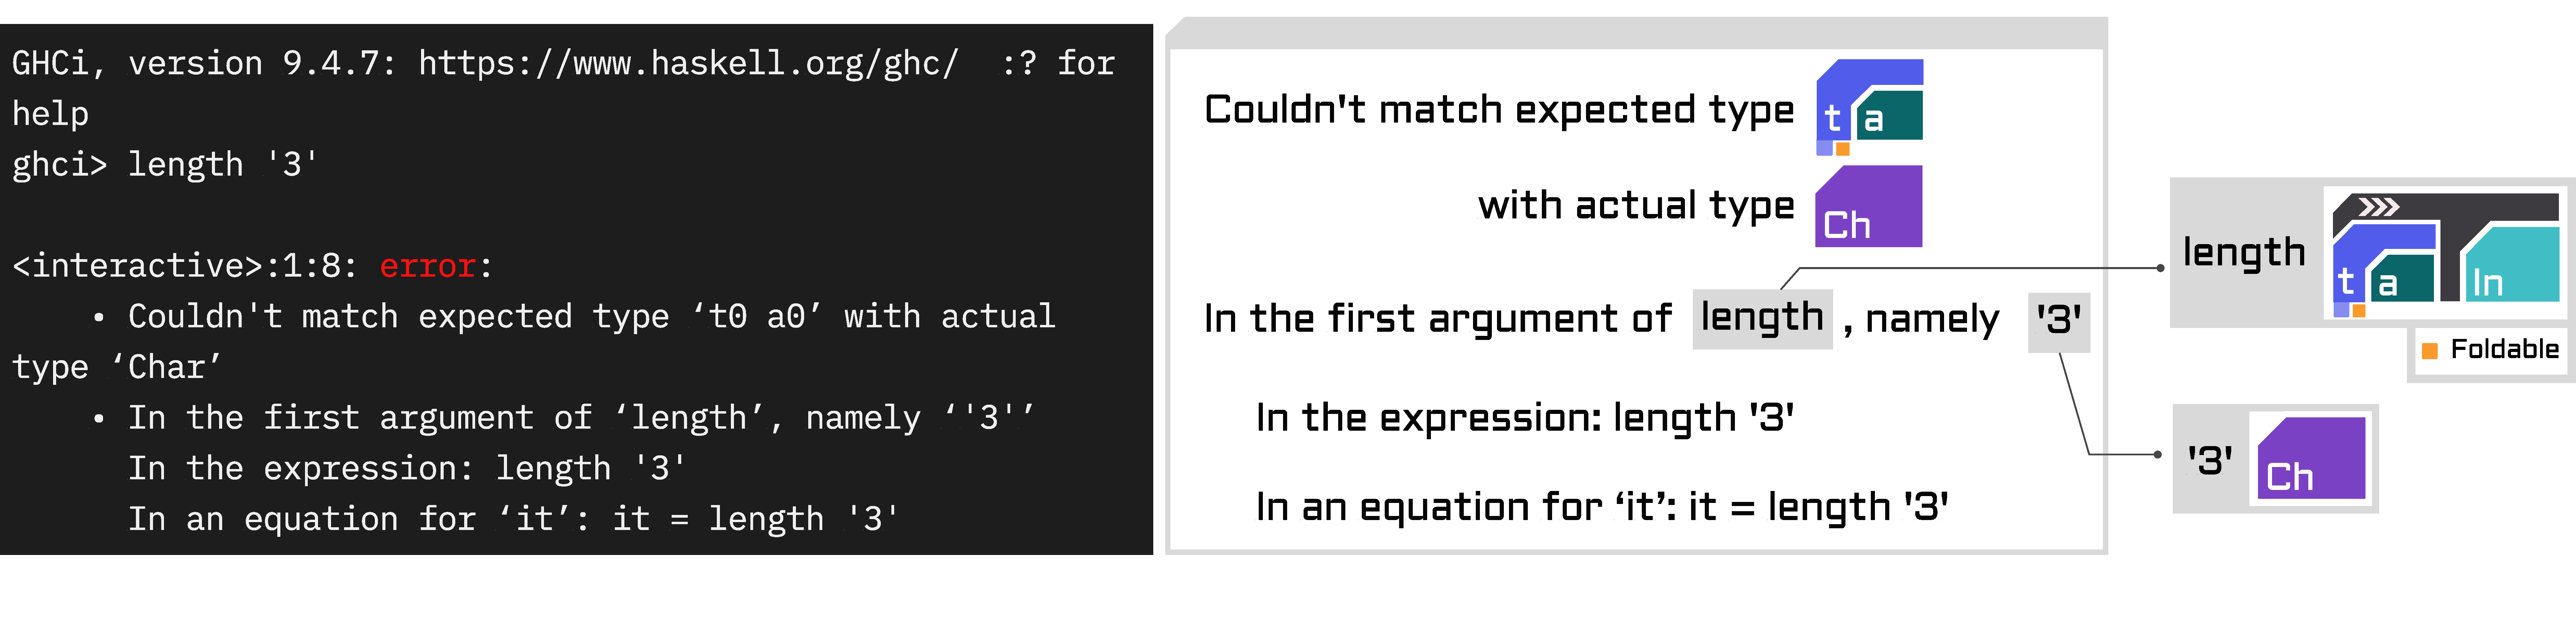
\includegraphics[width=\linewidth]{figures/Foldable}
  \caption{\label{fig:example-foldable} An example type error where a programmer mistakenly provided a \texttt{Char} instead of a \texttt{String} literal. {\bf Left:} Original type error. {\bf Right:} Type error with GeckoGraph}
\end{figure}

 We aim to investigate the challenges of using polymorphic types and explore how to improve their usability with visualization and modern Human-Computer Interaction (HCI) techniques. In this paper, we propose GeckoGraph, a graphical notation for types. GeckoGraph aims to complement traditional text-based type notation and make reading, understanding, and comparing types easier. GeckoGraph is prototyped and verified iteratively, leading to a design with visual clarity applicable to many programming contexts. 
 To evaluate its effectiveness, we conducted a large-scale user study comparing GeckoGraph with standard text-based type notation. To our knowledge, this represents the largest controlled user study on functional programming to date.
The results show no overall significant differences in task completion time or success rate. However, we observed a modest improvement in success rate among beginner participants. For the most challenging task, GeckoGraph improved success rates by 14.5\% for beginners and 11.2\% for less experienced users. These findings suggest that GeckoGraph has potential as a teaching and learning aid for polymorphic type systems.

\section{Type Systems in Functional Programming}

Functional programming languages have a rich history of embracing strong type systems and pioneering advanced type system features \cite{Milner1978-ob, MacQueen2020-qn, Hudak2007-kn}. In functional programming languages, type systems are often more expressive and provide stronger safety guarantees. They enable programmers to model program behavior rigorously and enforce correctness at compile time. Common characteristics of type systems in functional programming include structural typing, algebraic data types, parametric polymorphism, and type inference.

{\bf Structural typing} is often the primary approach for determining type equivalence and compatibility in functional programming languages (e.g., Elm and OCaml) and multi-paradigm languages (e.g., TypeScript). In contrast, nominal type systems are often predominant in Object-Oriented languages such as Java and C\# \cite{AbdelGawad2013-hh}. In nominal systems, two types are considered distinct even if they have identical structure but different names. In contrast, structural type systems consider types equivalent as long as their structures match, regardless of their names. This approach promotes flexibility, as types can be defined inline without introducing new names, and values are automatically valid for a type when they conform to the structure.  However, this lack of nominality can also make complex types harder to read and reason about. For instance, when encountering type errors, programmers can face two mismatched types with a complex structure, and understanding where exactly the root error is becomes a tedious task of string comparison (Fig. \ref{fig:structural}).

\begin{figure}[]
  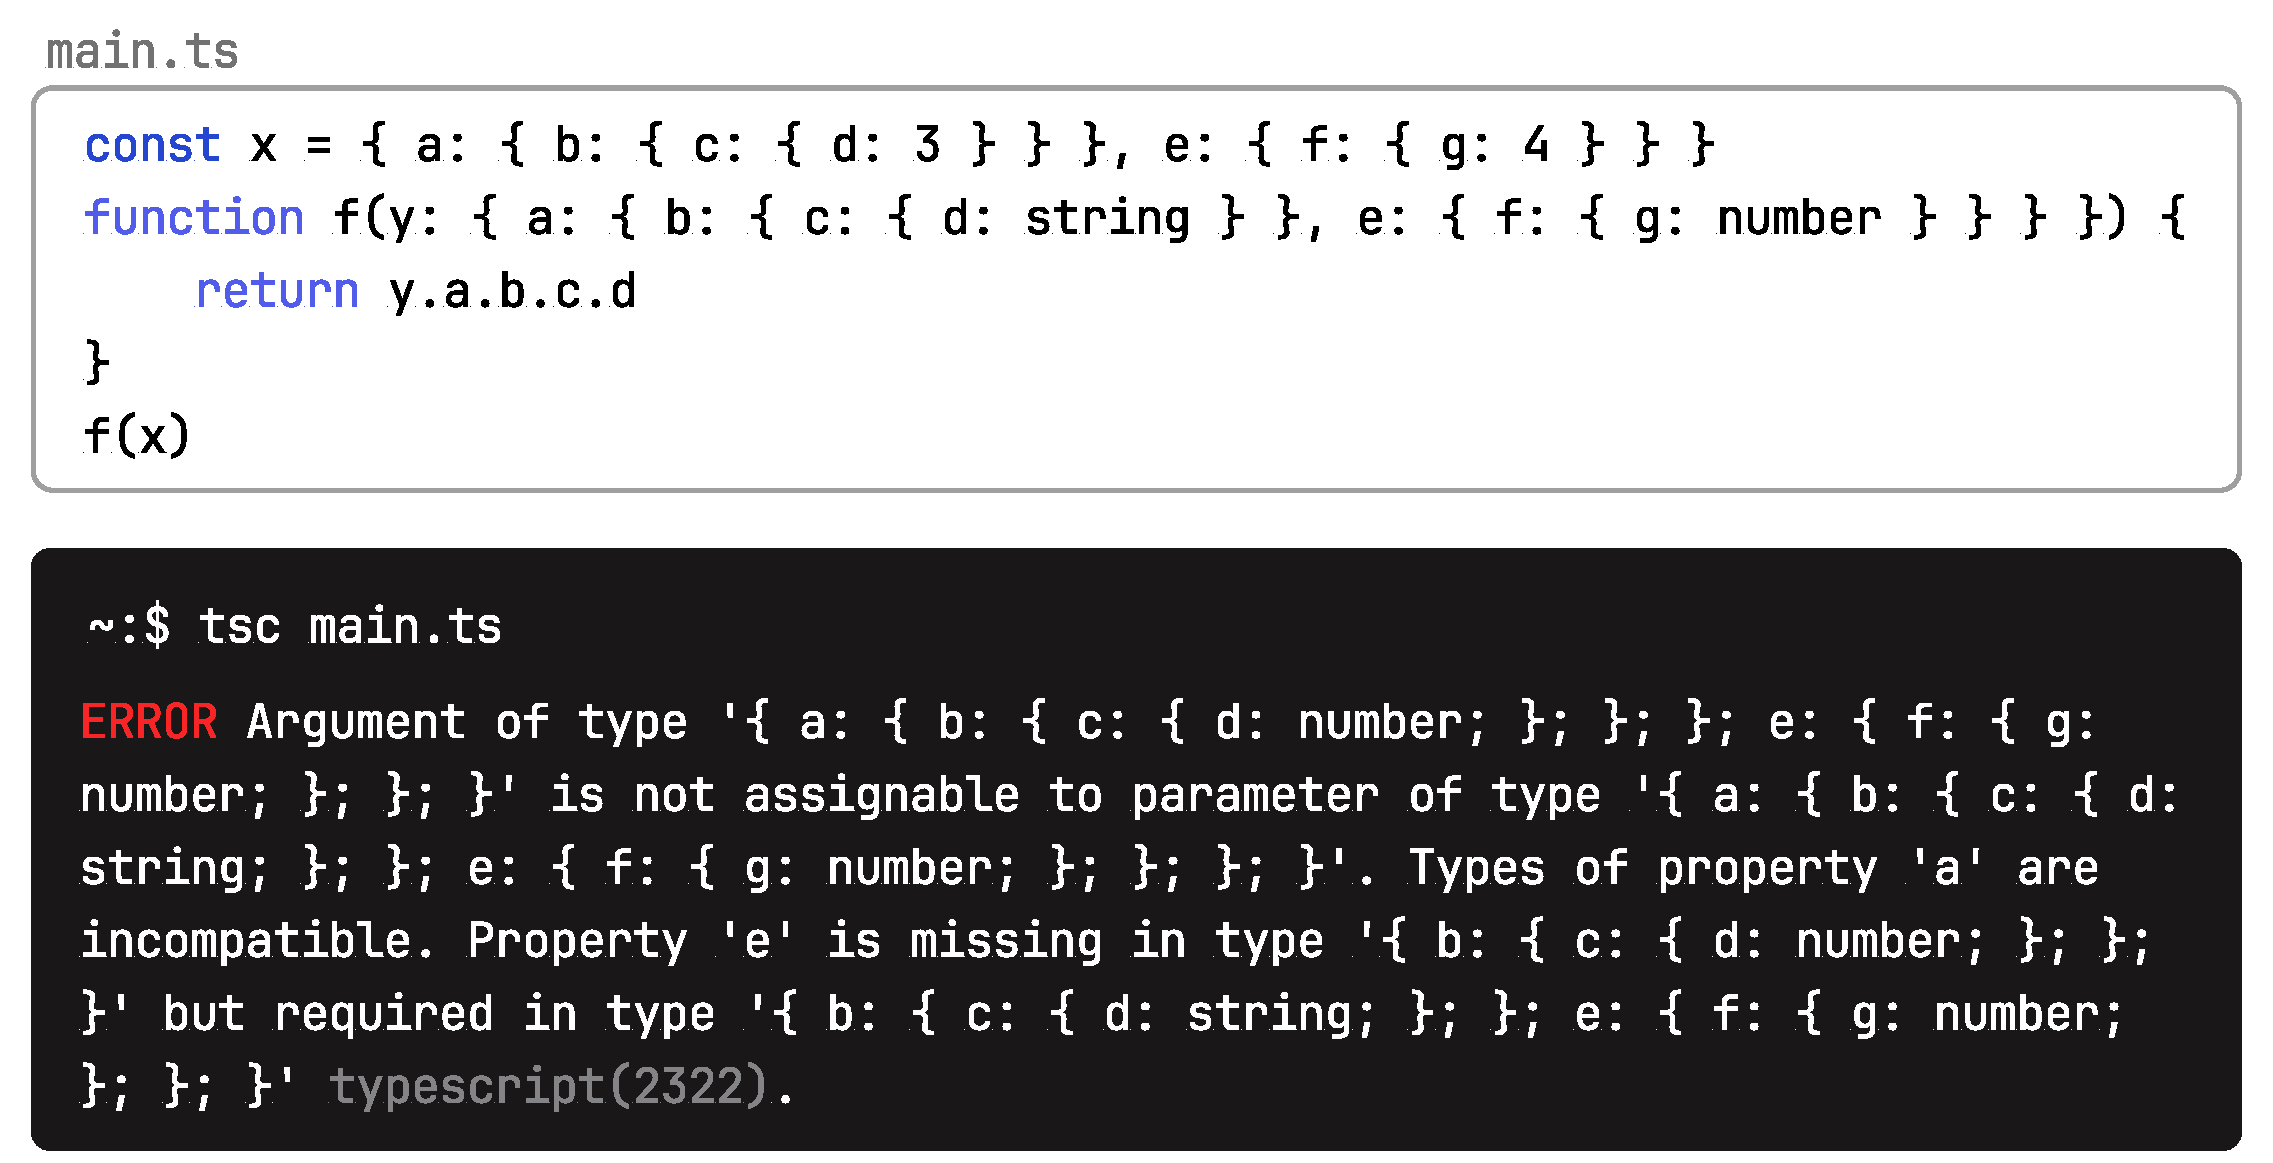
\includegraphics[width=\linewidth]{figures/structural}
  \caption{\label{fig:structural} Example of a TypeScript structural type error. (Top) The function \texttt{f} expects a parameter with a string field \texttt{d}, but the argument {\tt x} provides a numeric {\tt d}. (Bottom) The error message is dreadful to read.}
\end{figure}

{\bf Algebraic data types} (ADTs) \cite{Milner1978-qz} allow developers to construct complex types from simpler ones using sum and product operations. A {\bf sum type}, often called a tagged union, $A + B$, represents a type that can be a value of A or a value of B. Conversely, a {\bf product type} $A \times B$ represents a tuple type composed of two values of both {\tt A} and {\tt B}. This formalization allows precise and composable type construction for common data structures such as lists, tuples, and result types.
For example, in Haskell, types like \texttt{data Either a b = Left a | Right b} and \texttt{data Maybe a = Nothing | Just a} provide basic building blocks for error handling, and the type \texttt{data List a = [] | a : List a } provides a succinct recursive definition for lists. This illustrates the expressive power of ADTs. However, in practice, type definitions can grow to be complex structures, for instance \texttt {Maybe (Either [Maybe a] (Either a String))} as programs grow, causing difficulties to interpret and maintain. 


{\bf Parametric polymorphism} (often called generics) allows functions and data structures to operate uniformly across different types. For instance, in Haskell, the function \texttt{head :: [a] -> a}, taking a list as input and returning the first element, is a polymorphic function that works on lists of any type; integers, strings, and functions are all valid candidates for the generic variable \texttt{a}.  It provides a strong and principled form of abstraction, enabling code reuse without sacrificing type safety.

However, parametric polymorphism also increases cognitive load: programmers must mentally track type variables and reason about how concrete types are instantiated during function application. This task becomes more challenging when functions involve multiple type variables. An example would be the foldM function: \texttt{foldM :: (Monad m) => (a -> b -> m a) -> a -> [b] -> m a}. The challenge of reading and understanding polymorphic types is more serious for novice users \cite{Jun2000-ec, Jun2000-yu}.



{\bf Type inference}, or implicit typing, reduces the need for explicit type annotations by allowing the compiler to deduce types automatically.
Most modern languages employ some level of inference. For instance, Java’s var keyword (introduced in version 10) infers variable types at compile time based on their assigned values \cite{Java_Developers2023-an}, saving programmers from writing redundant type declarations, such as \textit {Car car = new Car()}.

Functional languages such as Haskell and ML go further, using global type inference \cite{Damas1982-zw} to check entire programs without requiring explicit annotations. While this improves conciseness, it can reduce code readability and produce complex error messages. Many programmers, therefore, choose to write explicit type signatures for clarity, even when inference is available.




{\it To summarize}, the type systems of functional programming languages provide rigorous tools for specifying and enforcing program behavior. By encoding system constraints directly in types, they prevent many classes of runtime errors. However, this rigor introduces trade-offs: a steeper learning curve and less flexibility for exploratory or prototype development. In the following sections, we explore how GeckoGraph supports these type-system features by visualizing type-level information that is often implicit or difficult for humans to interpret.


\section{GeckoGraph}

GeckoGraph is a visual notation for type annotations in statically typed programming languages. It is intended to work tangibly with text-based annotations but uses colors, shapes, and symbols to make structures of types easy to identify at a glance. In this section, we describe the design of GeckoGraph and highlight some unique benefits of programming with GeckoGraph.

\subsection{Design of GeckoGraph}
The design of GeckoGraph focuses on visualizing types in functional languages (e.g., Haskell, ML). In this paper, we use Haskell as an example. As illustrated in this section, it can express basic types, polymorphic types, algebraic data types, type classes, and a few advanced type-level features. However, GeckoGraph can also be used in imperative and multiparadigm languages such as TypeScript and Rust. We provide a GeckoGraph visualization tool available online for multiple languages \cite{Fu2025-ka}.

We identified three main design goals for GeckoGraph based on the challenges of using polymorphic types~\cite{Jun2000-ec, Jun2000-yu} and how programmers tend to use type annotations to support their programming tasks~\cite{Justin_Lubin2021-yy}, as follows. 

\paragraph{\textbf{(D1) Easy to learn}}\label{goal1} GeckoGraph should take little to no effort to learn. The rules to translate a text-based type notation to GeckoGraph should be minimal. Where possible, GeckoGraph should be intuitive to programmers who are familiar with text-based type notation.

\begin{figure}[!h]
  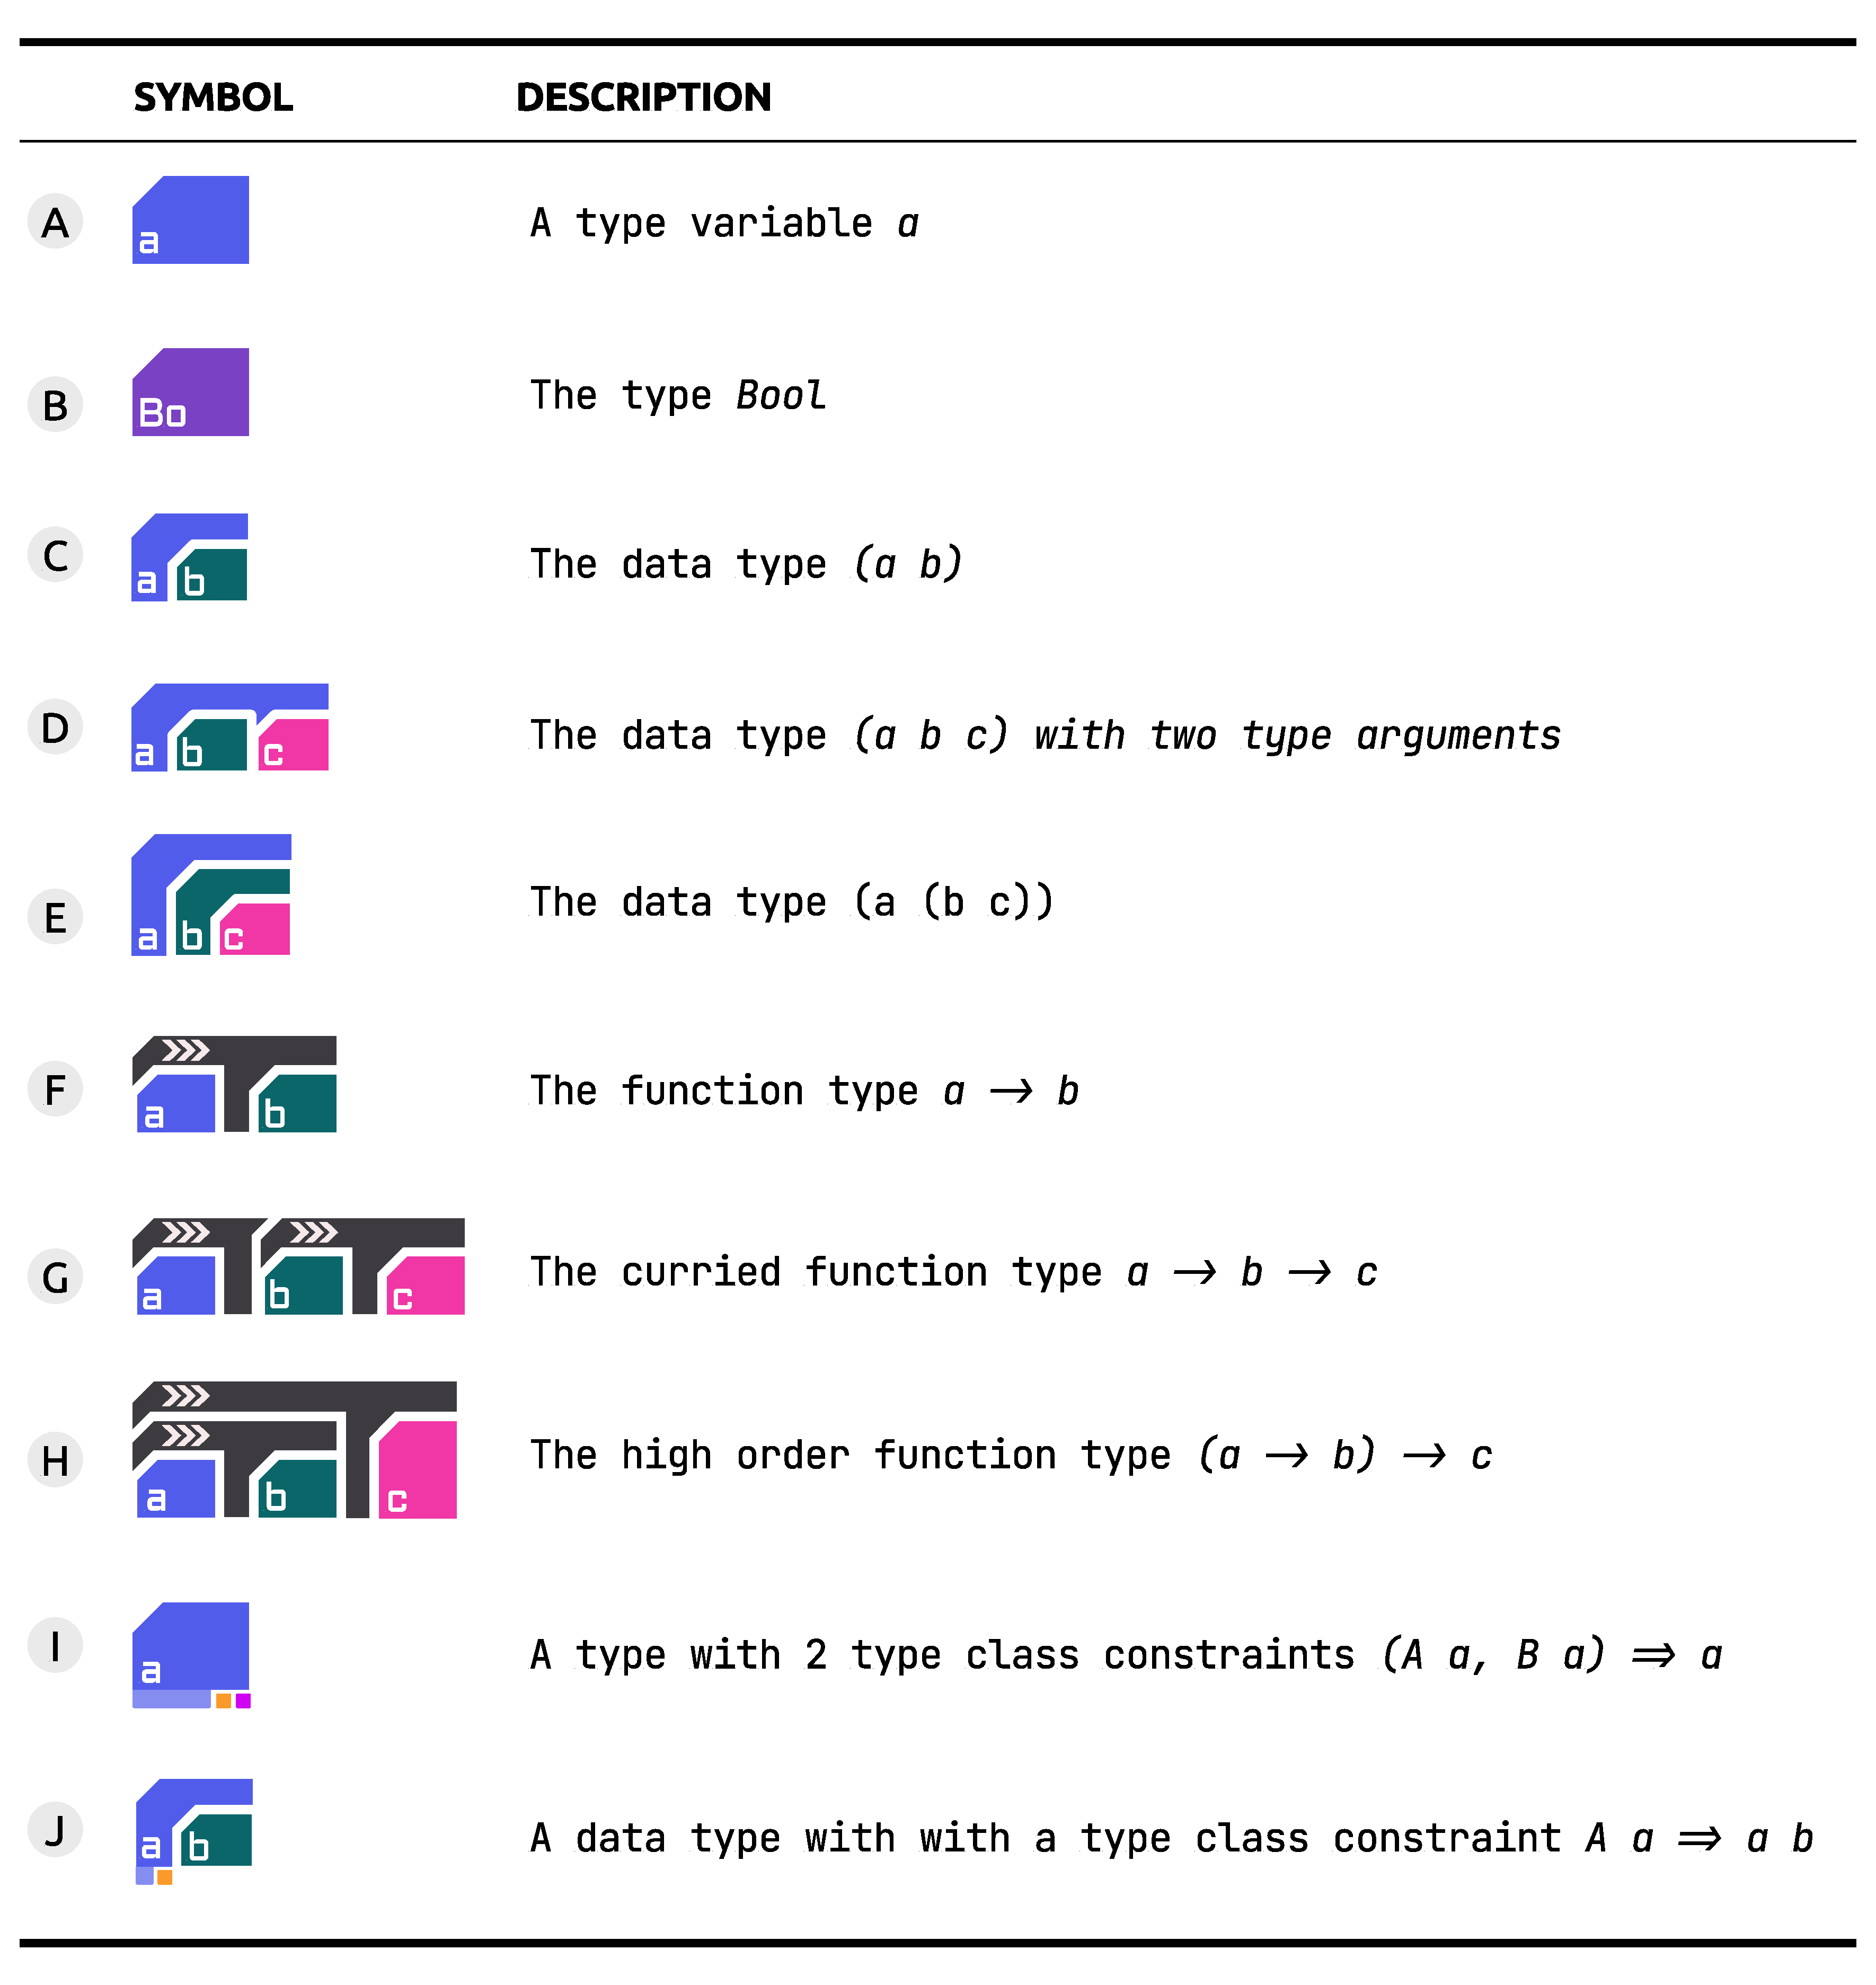
\includegraphics[width=\linewidth]{figures/Design}
  \caption{
        \label{fig:design}
        Examples of various types as represented in GeckoGraph, including type variables (A) and concrete types (B). Data types (C, D, E), function types (F, G, H), and type classes (I, J).
  }
\end{figure}

\paragraph{\textbf{(D2) Easy to parse for humans}}  \label{goal2} GeckoGraph should make the task of reading and understanding type notation easy. It should emphasize the less obvious properties of a type signature. GeckoGraph should eliminate the need for mental backtracking, such as counting opening and closing parentheses and remembering which type classes are required on which variables. 

\paragraph{\textbf{(D3) Optimized for comparing and searching}} \label{goal3} GeckoGraph aims to make the task of comparing two types easy, especially to make subtle differences in text-based notation harder to miss. This also includes the task of choosing an ideal function from a list of potential functions. For example, programmers search for a desired function from a documentation site with only partial knowledge of its type (e.g., the arity of a function, containing a known type, or type class requirements). 

Motivated by the design goals, we designed GeckoGraph with the following features and construction rules (Fig. \ref{fig:design}):

\paragraph{Simple Types} 
Simple types, such as type variables and concrete types, are displayed in a cell 
\includegraphics[height=1em]{figures/SimpleType}: a solid-colored rectangular box with an angled corner on the top left. Each type identifier encodes a distinct color hue of the cell. Its first 1 or 2 letters are displayed inside the cell at the bottom left to provide familiarity (design goal \ref{goal1}) and a strong secondary encoding. The angled corner in the top left provides visual separation between two cells, even when the same color cells are next to each other, allowing GeckoGraph to be zoomed out to extremely small sizes (Section \ref{subsec:space}) without suffering readability (design goal \ref{goal2}).



\paragraph{Algebraic Data Types}
GeckoGraph displays an algebraic data type as a larger cell, where the type constructor half encloses its arguments: 
\includegraphics[height=1em]{figures/DataType.png}. The arguments are aligned in the bottom right of the cell. Two distinct visual dimensions are used to provide additional visual clarity (design goal \ref{goal2}). Data types containing more arguments (e.g., \texttt{ a b c} or \texttt{(a b) c}) will expand horizontally 
\includegraphics[height=1em]{figures/DataTypeWide.png}. Data types that are nested (e.g. \texttt{ a (b c)}) will grow taller 
\includegraphics[height=1.2em]{figures/DataTypeNested.png}. This distinction accommodates our design goal \ref{goal3}. Note that the height of GeckoGraph grows only upwards, but not downwards. Not only does this allow GeckoGraph to be more efficient in its space usage, but it also allows the legend text to be consistently aligned at the bottom and can be read as though it is a text-based type notation (design goal \ref{goal1}).  

\paragraph{Function Types}
Functions are the fundamental building blocks of functional programming languages, and function types are ubiquitous and the most important in type-level programming. In Haskell, \texttt{(->)} is defined as an infix type operator with right associativity to provide succinct type annotations. GeckoGraph preserves this syntax feature to make the notation more intuitive (design goal \ref{goal1}): the 2 arguments of a function type in GeckoGraph are placed on both sides of the cell 
\includegraphics[height=1em]{figures/Function.png}. A special function indicator (\texttt{$>>>$}) is displayed at the top of the cell. 

Curried functions (e.g., \texttt{ a -> b -> c}) are displayed as two cells of functions merged together 
\includegraphics[height=1em]{figures/Curry.png}. It appears as if the second function covers the right half of the first function, indicating that the second function is the return type of the first. Regular high-order functions (e.g., \texttt{(a -> b) -> c}) follow the rules of functions and nested data types 
\includegraphics[height=1.2em]{figures/HOF.png}. The placement of function indicators aims to make it easy to find desired functions in the documentation site based on function arity and higher-order functions (design goal \ref{goal3}). It is easy to tell high-order functions from the vertical position of the function indicators. Similarly, it is easy to count the arity of a function by counting the number of function indicators at the outer layer. For example, in Fig. \ref{fig:indicator}, the outer layer function indicators (the ones colored in the lightest shade of gray) suggest a ternary function. The two argument types and the return type are all functions.

\begin{figure}[h]
  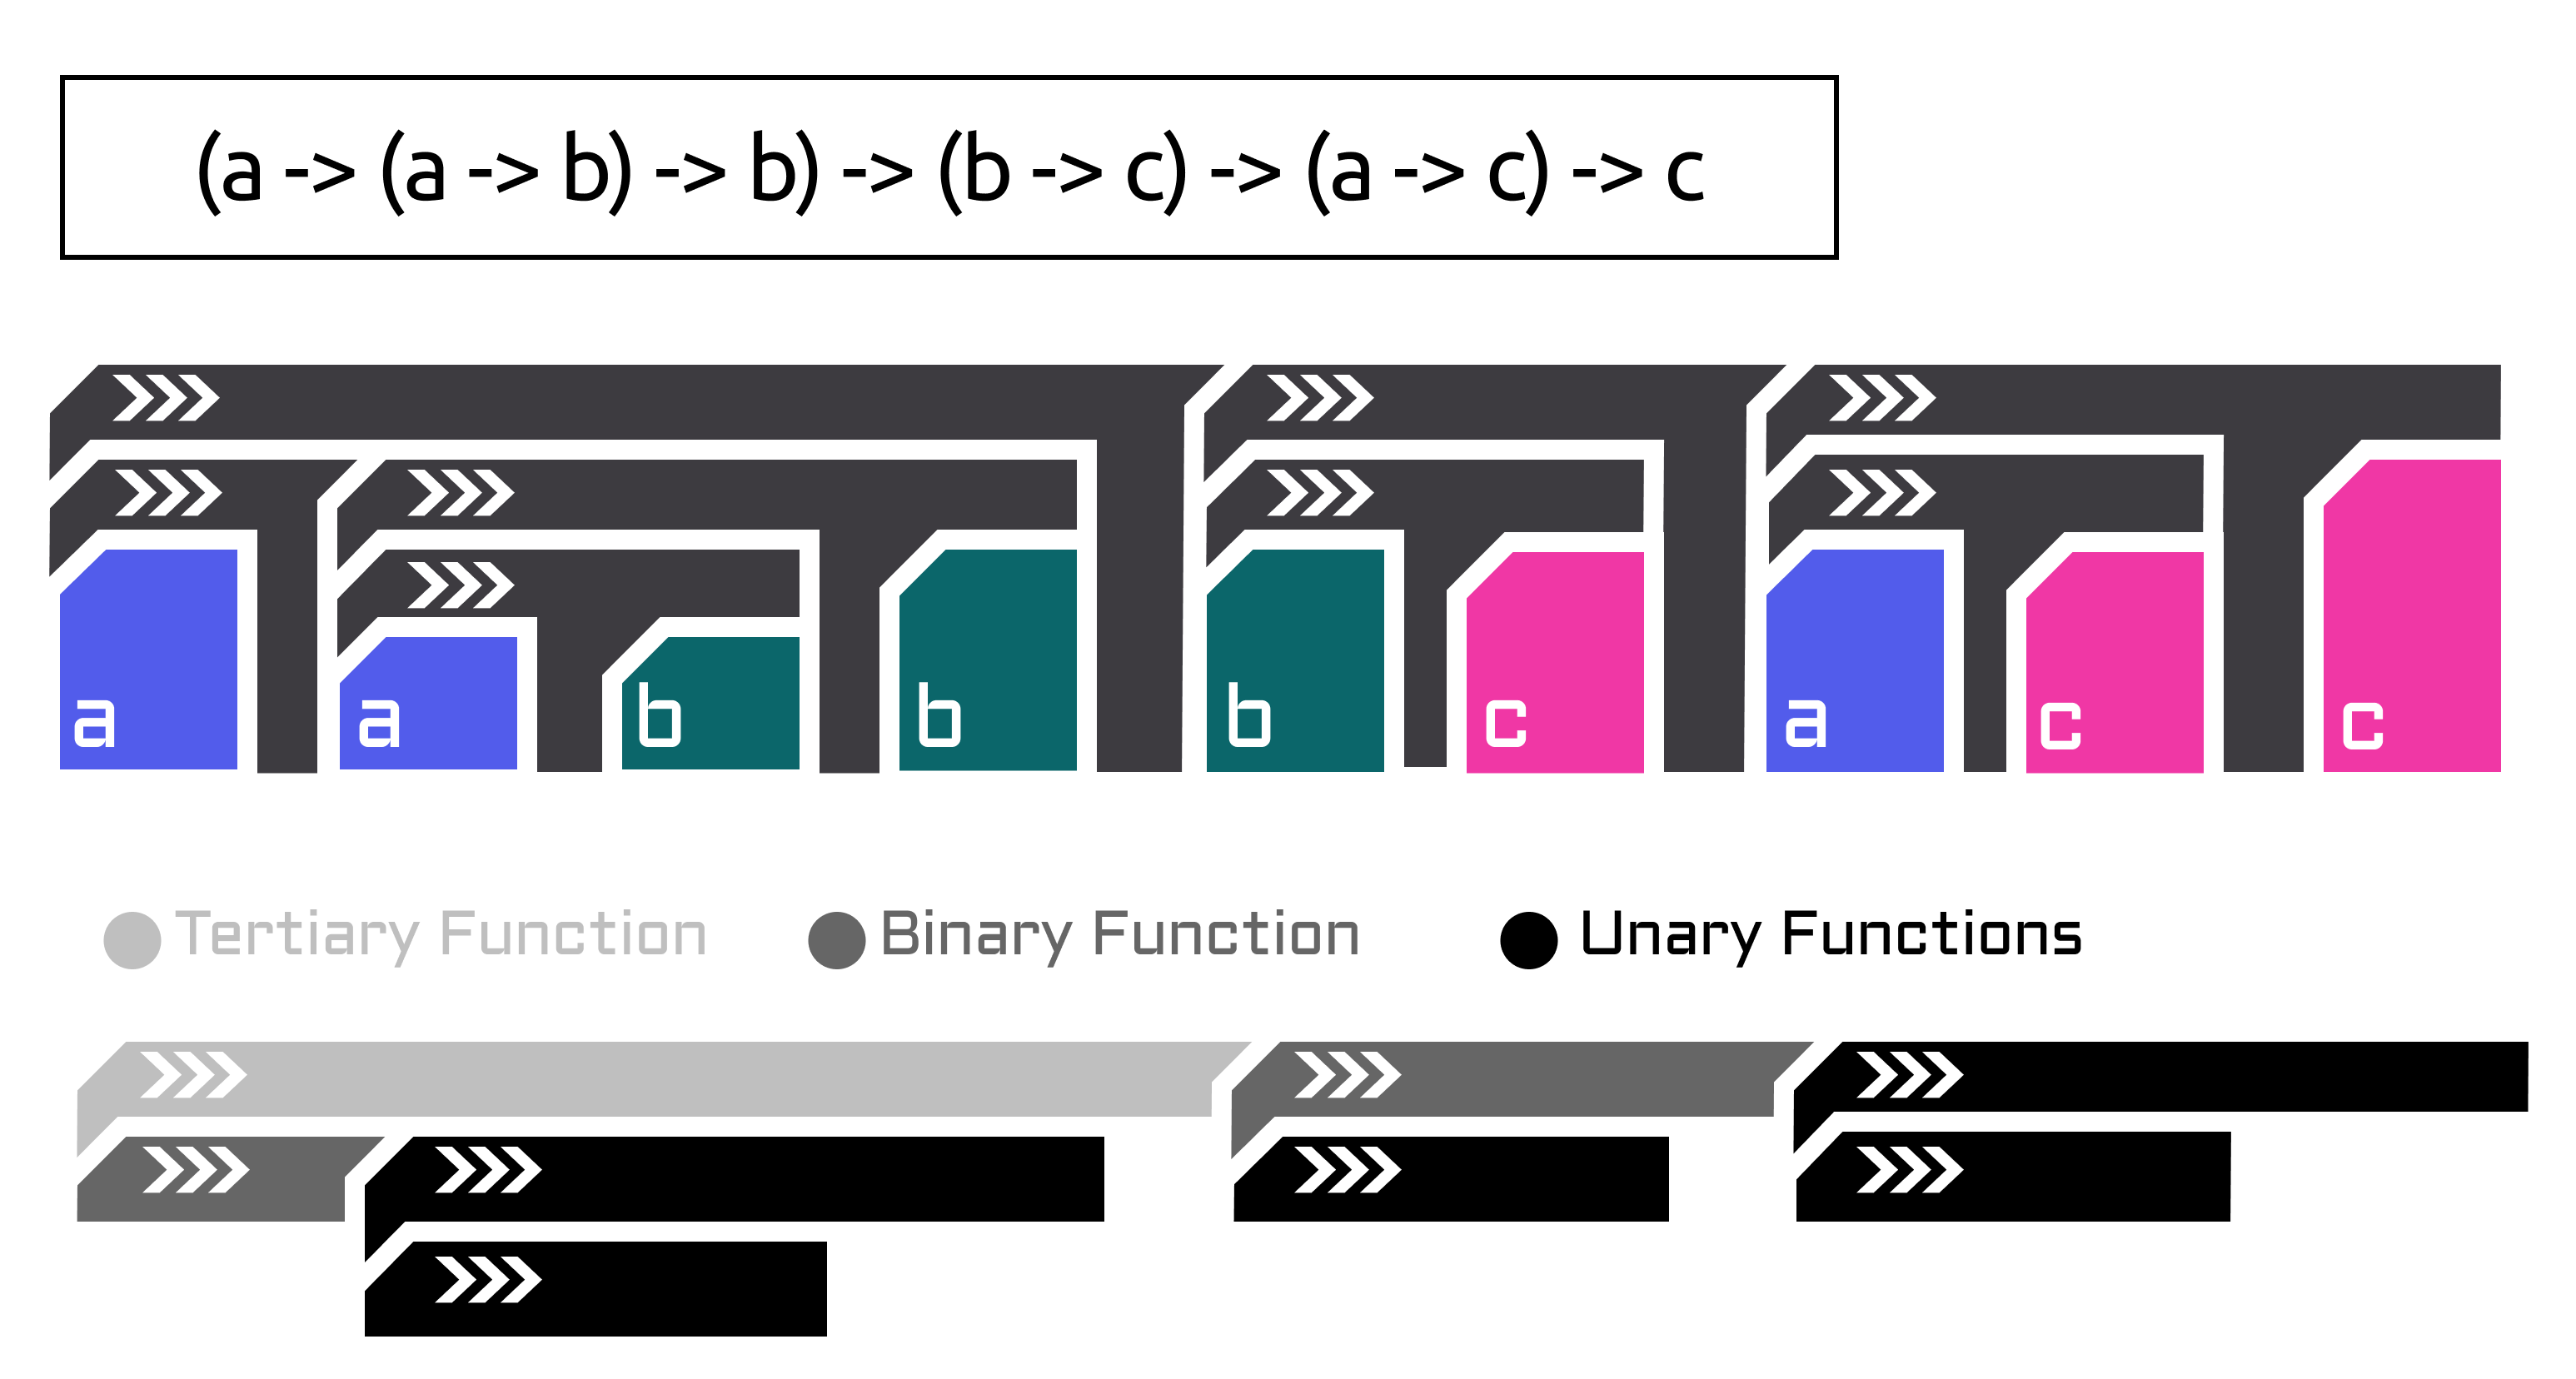
\includegraphics[width=\linewidth]{figures/Indicator}
  \caption{
        \label{fig:indicator}
        An example of the visual hierarchy of the function indicator. The function indicator can be used to easily identify the arity of a function type by counting the connecting function indicators. For higher-order functions where functions are arguments or return values of other functions, it is very easy to see the ``level" of functions. 
  }
\end{figure}

 
\paragraph{Type Classes} 
Type classes are an intrinsic part of Haskell \cite{Hudak2007-kn}, and many other functional languages. In GeckoGraph, the type classes (e.g., \texttt{ (A a, B a) => a}) are indicated in the extended area below one or more GeckoGraph cells 
\includegraphics[height=1.2em]{figures/TypeClass.png}. Each type class required on a type variable displays as a square indicator aligned on the right of the extended area. In GeckoGraph, a type-class glyph is embedded in every type variable that requires this class. This means when displaying the type \texttt{(==) :: Eq a => 
a -> a -> Bool} in GeckoGraph, the constraint \texttt{Eq} appears in twice on both occurrences of the type variable \texttt{a}. 

The GeckoGraph type class's design promotes the type class placements rather than the type class names. Programmers can easily see where and how many type classes are required, but they may need an extra step (global legends of the color mapping or a pop-up window) to identify the name of the type class. We believe that this is a well-justified trade-off. The strength of this approach lies in situations when the type class context is complex. When reading a type \texttt{(A a, A c, B a, B b, C b) => a -> b -> c}, programmers may need to switch back and forth to remember which type classes are needed on which variable. In GeckoGraph, type classes are explicitly displayed under the type variable cell,  minimizing programmers' effort to associate each type variable with all its type classes (design goal \ref{goal2}). 


\subsection{Key Design Criteria of GeckoGraph}\label{sec:benefits}

GeckoGraph was designed through many different iterations. Many research methods were used to verify ideas, including prototyping, cognitive walk-throughs, and formative studies. We discuss some notable visual dimensions in GeckoGraph and their justifications.


\paragraph{Visual Dimensions of GeckoGraph}

\textbf{The colors of GeckoGraph} help programmers to see the permutation of type variables in the input and output of a function. A recent review \cite{Zeng2023-jz} of 59 graphical perception articles showed that combining solid color hue in a filled shape provides stronger visual perception for nominal data such as type identifiers. GeckoGraph uses a qualitative color scheme from ColorBrewer \cite{Harrower2003-vu} to encode symbolic values of types. One example of GeckoGraph's use of color is the ``rotation" function  (Fig. \ref{fig:rotate}) in the user study (Section \ref{sec:evaluation}). With text-based type notation, programmers often rely on mnemonic devices such as alphabetic ordering or naming conventions. For example, the rotation function \texttt{f2 :: Zero a b c d -> Zero b c d a} appeared in the evaluation (Section \ref{sec:evaluation}), shuffles the type arguments one step to the left. The purpose of this function becomes less recognizable if changed to \texttt{f2 :: Zero e v m h -> Zero v m h e}. 

\begin{figure}[]
  \includegraphics[width=0.6\linewidth]{figures/rotate}
  \caption{\label{fig:rotate} The `f2' function in the user study. It shuffles the type arguments one step to the left, and the leftmost argument wraps around to be the rightmost.}
\end{figure}

\textbf{The horizontal axis of GeckoGraph} is often helpful for identifying differences in function arities. For example, in Fig. \ref{fig:add3}, the programmer intended to implement a function that sums 3 integers. In the implementation, the programmer missed a \texttt{(+)} function at the end; the resulting function type is largely different in length. It is also clear that the function needs to apply to one more binary function to satisfy the length requirement.  

\begin{figure}[h]
  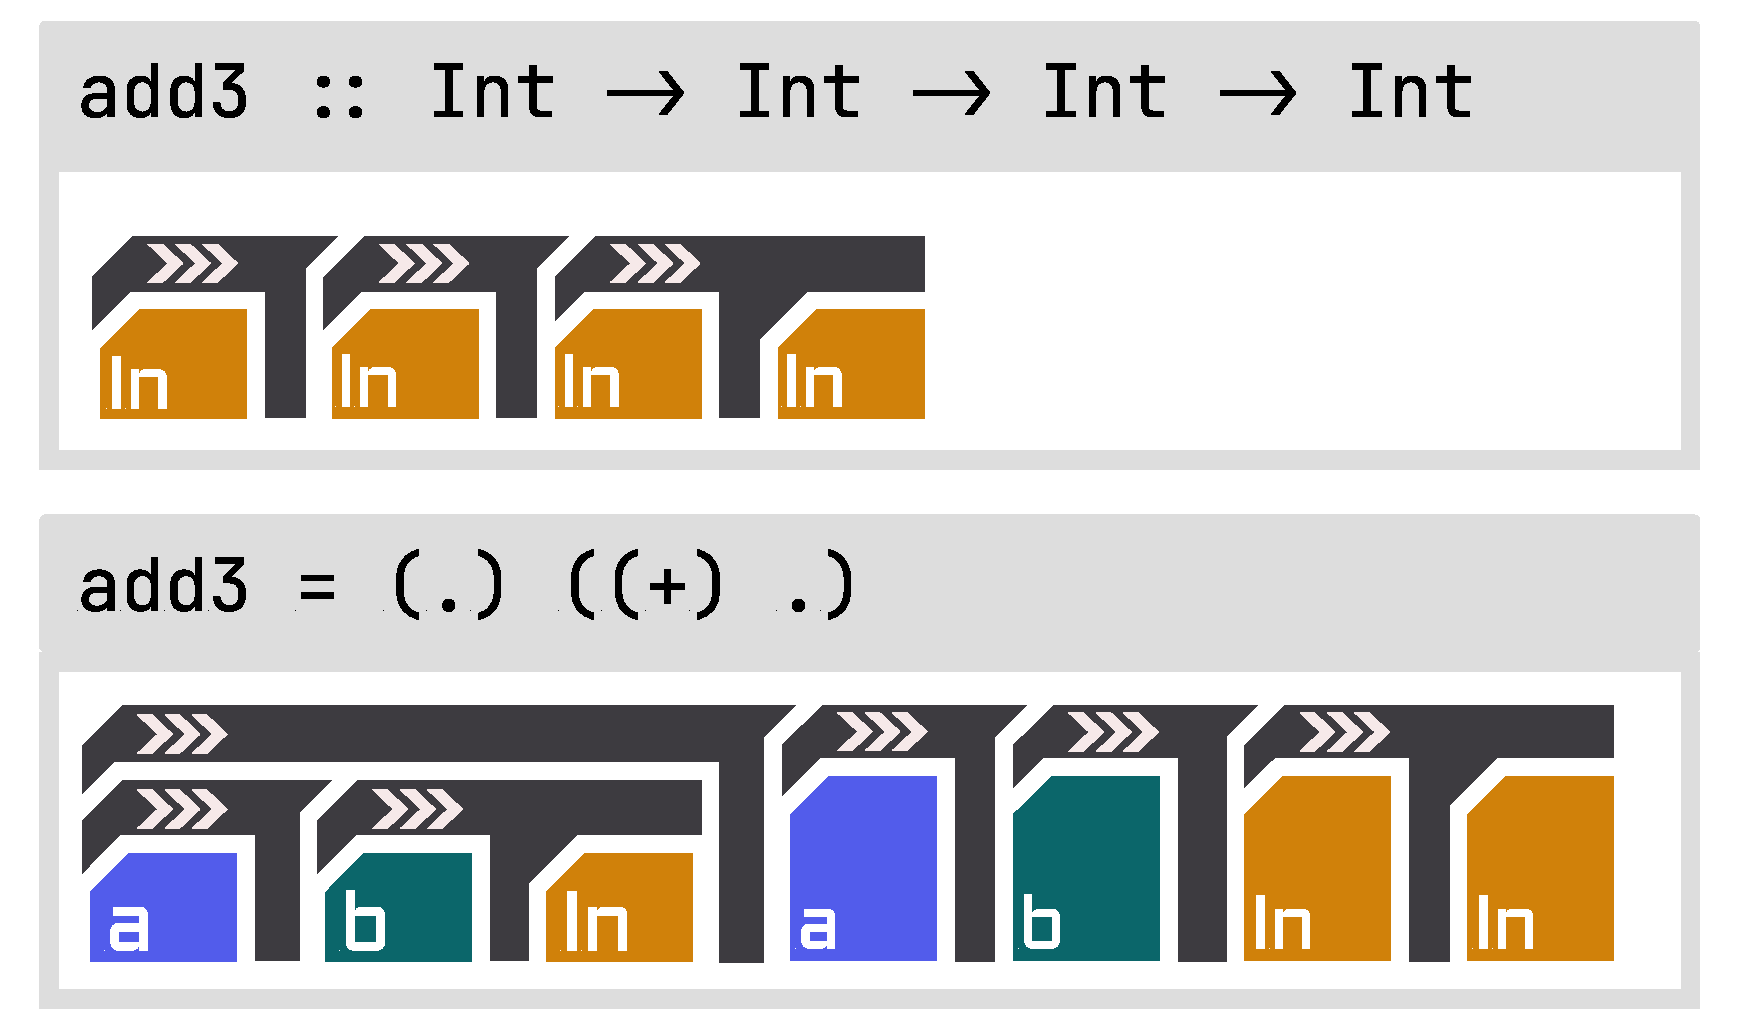
\includegraphics[width=0.6\linewidth]{figures/Add3}
  \caption{\label{fig:add3} An implementation of function \texttt{add3} but the author missed an (+) from the correct implementation (.) ((+) .) (+). GeckGraph highlights the difference in arity and reveals that a binary function is needed on the right-hand side for the arity to match. }
\end{figure}

\textbf{The vertical axis of GeckoGraph} often helps identify the number of levels in a nested complex type. This can often be very useful when inspecting mismatched types where data types are nested at different levels. Common examples include when programmers forget to apply the value to ``return" in a monadic block or to use \texttt{liftIO} to cast an \texttt{IO} effect. In Fig. \ref{fig:maybe}, the uses of \texttt{return} are excessive. It can be easily identified by examining the difference in the vertical layers of the two types. In text-based type notation, this is distinguished by different pairs of parentheses. However, parenthesis is an overloaded syntax in type notation. In Haskell, parentheses are used to enclose tuples \texttt{(a, b)}, specify the fixity \texttt{ (a -> b) -> c}, or have no effect \texttt{a -> (b -> c)}.

	
\begin{figure}
  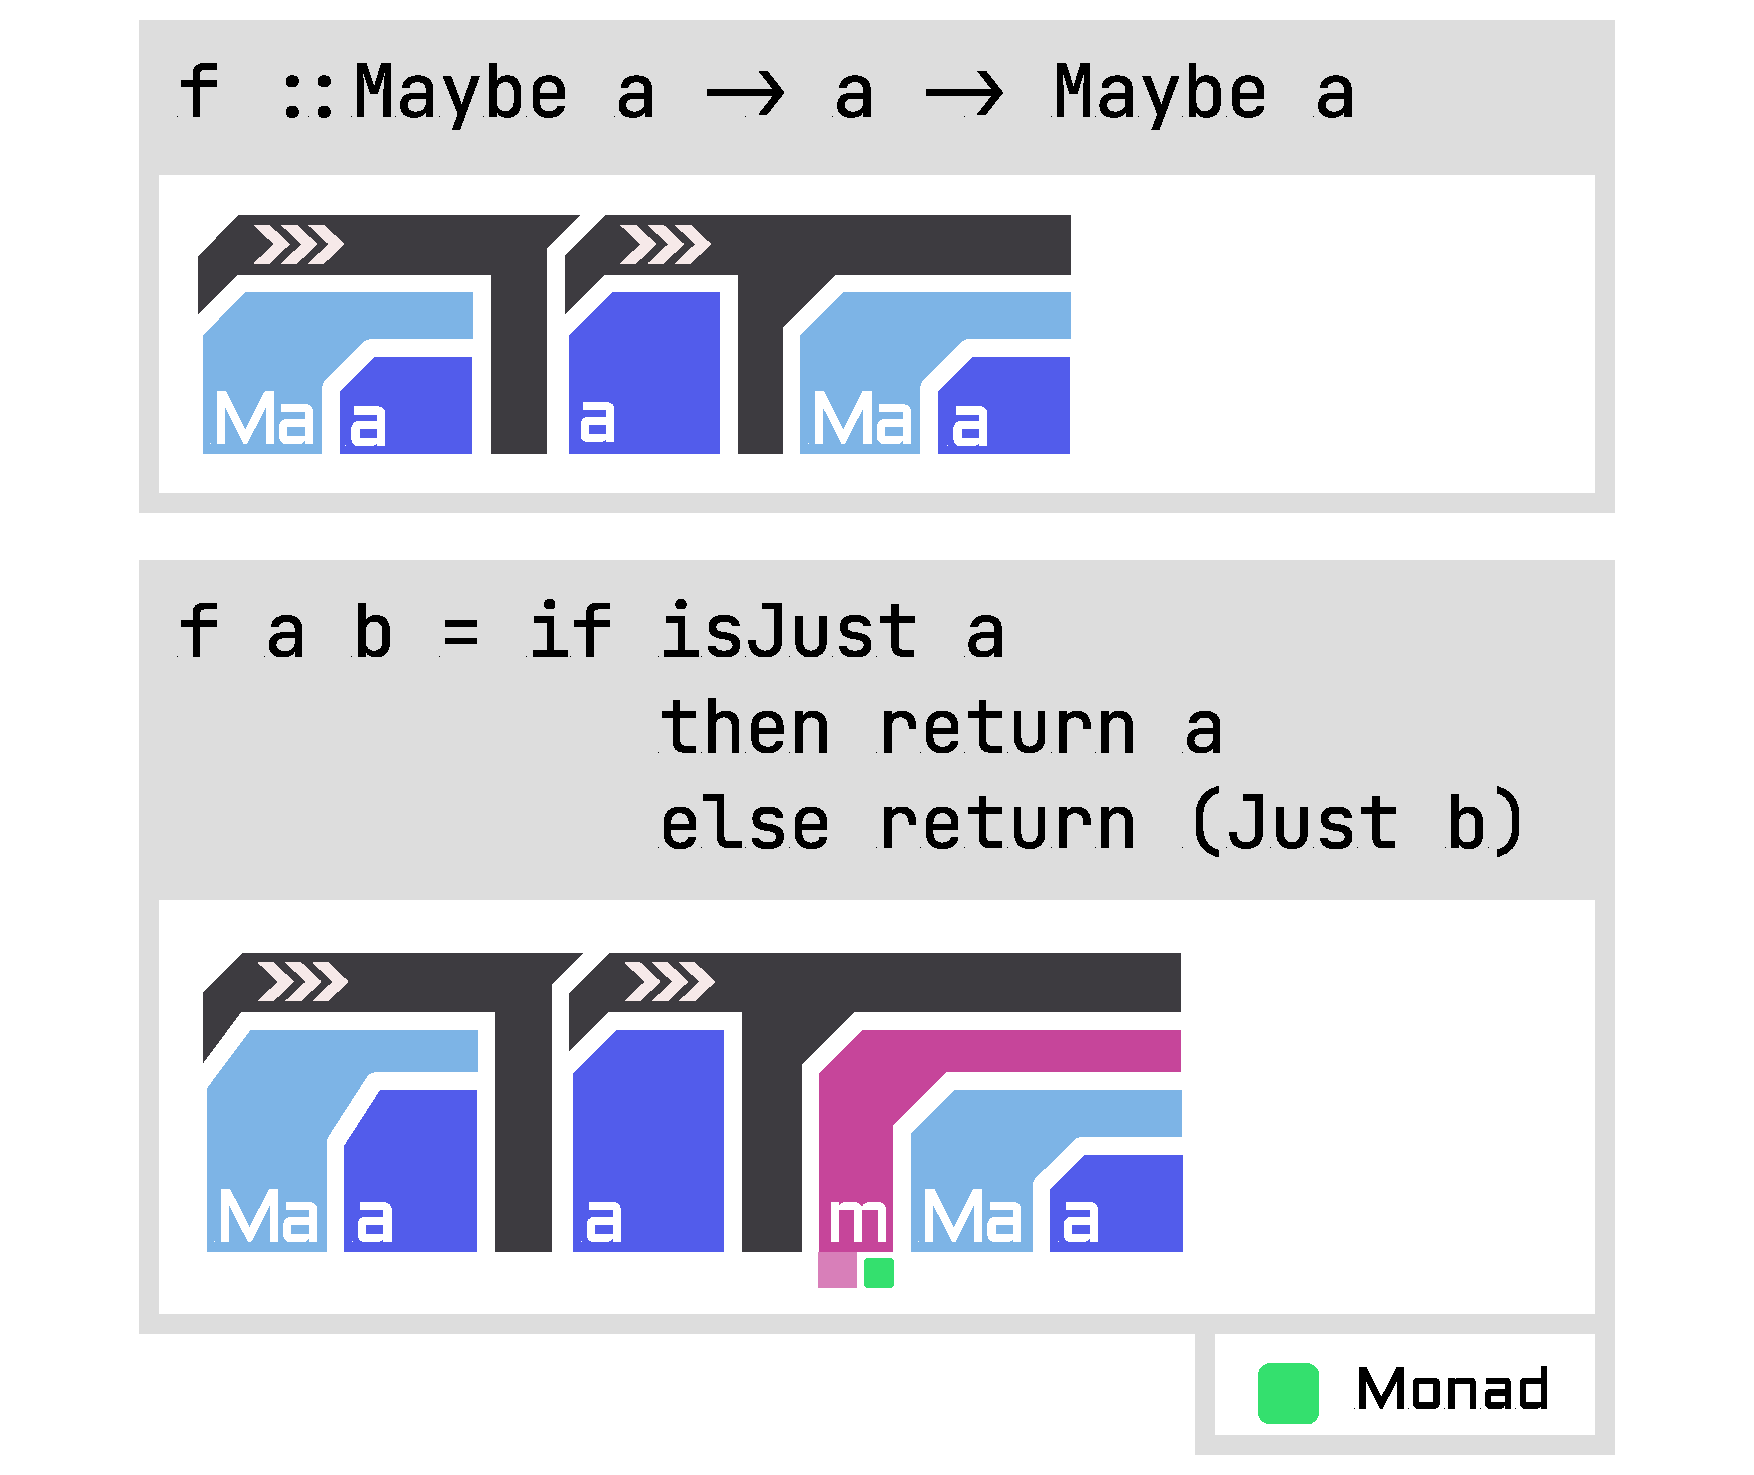
\includegraphics[width=0.6\linewidth]{figures/Maybe}
  \caption{\label{fig:maybe} The function \texttt{f} is planned to have the type \texttt{Maybe a -> a -> Maybe a}. The programmer mistakenly applied the result to the \texttt{return} function, making the result inside a Monad instance.  GeckoGraph reveals the difference in the ``layers" of types. }
\end{figure}

\paragraph{Support Advanced Type Features}
The design of GeckoGraph enables the visualization of many advanced type-level features. \textbf{Kind visualization}: The kind system \cite{Jones1995-lm} is used in Haskell to indicate whether a type is a type constructor (e.g., [], Maybe) or a type constant (e.g., Bool, Char). Because of this, kind is often described as the type of types. GeckoGraph infers the {\it kind} of type variables and consistently displays this information. For example, in Fig. \ref{fig:advanced} (A), the variable \texttt{a} is inferred to have the kind \texttt{* -> *} because of its use on the right-hand side. GeckoGraph respects this {\it kind} information and displays the same kind level on the first occurrence of \texttt{a}, but over an empty structure, indicated using a dotted outline. \textbf{Qualified constraints}: GeckoGraph's type class notation naturally extends to support qualified constraints. In the type \texttt{forall b. A (a b) => a b}, GeckoGraph shows the scope type class requirement on \texttt{a b} (Fig. \ref{fig:advanced} B).
\textbf{Multiple Parameter Type Class}:  GeckoGraph supports multiple parameter type classes by using multiple shapes with the same color hue to indicate the different parameters of the same type class. For example, for the type \texttt{A a b => a b},  GeckoGraph shows that the variables a and b both need an A class, but they are the different parameters of A (Fig. \ref{fig:advanced} C).

\paragraph{Provide Precise Interactivity}
Modern programming environments often allow programmers to mouse over part of the source code to query detailed information, such as definition, references, or documentation. However, with text-based source code, it is often hard to distinguish whether programmers want the most specific fragment under the cursor or larger blocks. Because of its graphical layout, GeckoGraph allows programmers to precisely select which part of a type signature they intend to query, that is, in Fig. \ref{fig:advanced} (D) when the user mouses over the type class box (orange square) under the second occurrence of \texttt{a} the type class it represents is revealed in detail, a specific query that is hard to execute with point and click over text based type annotation.

\begin{figure}[h]
  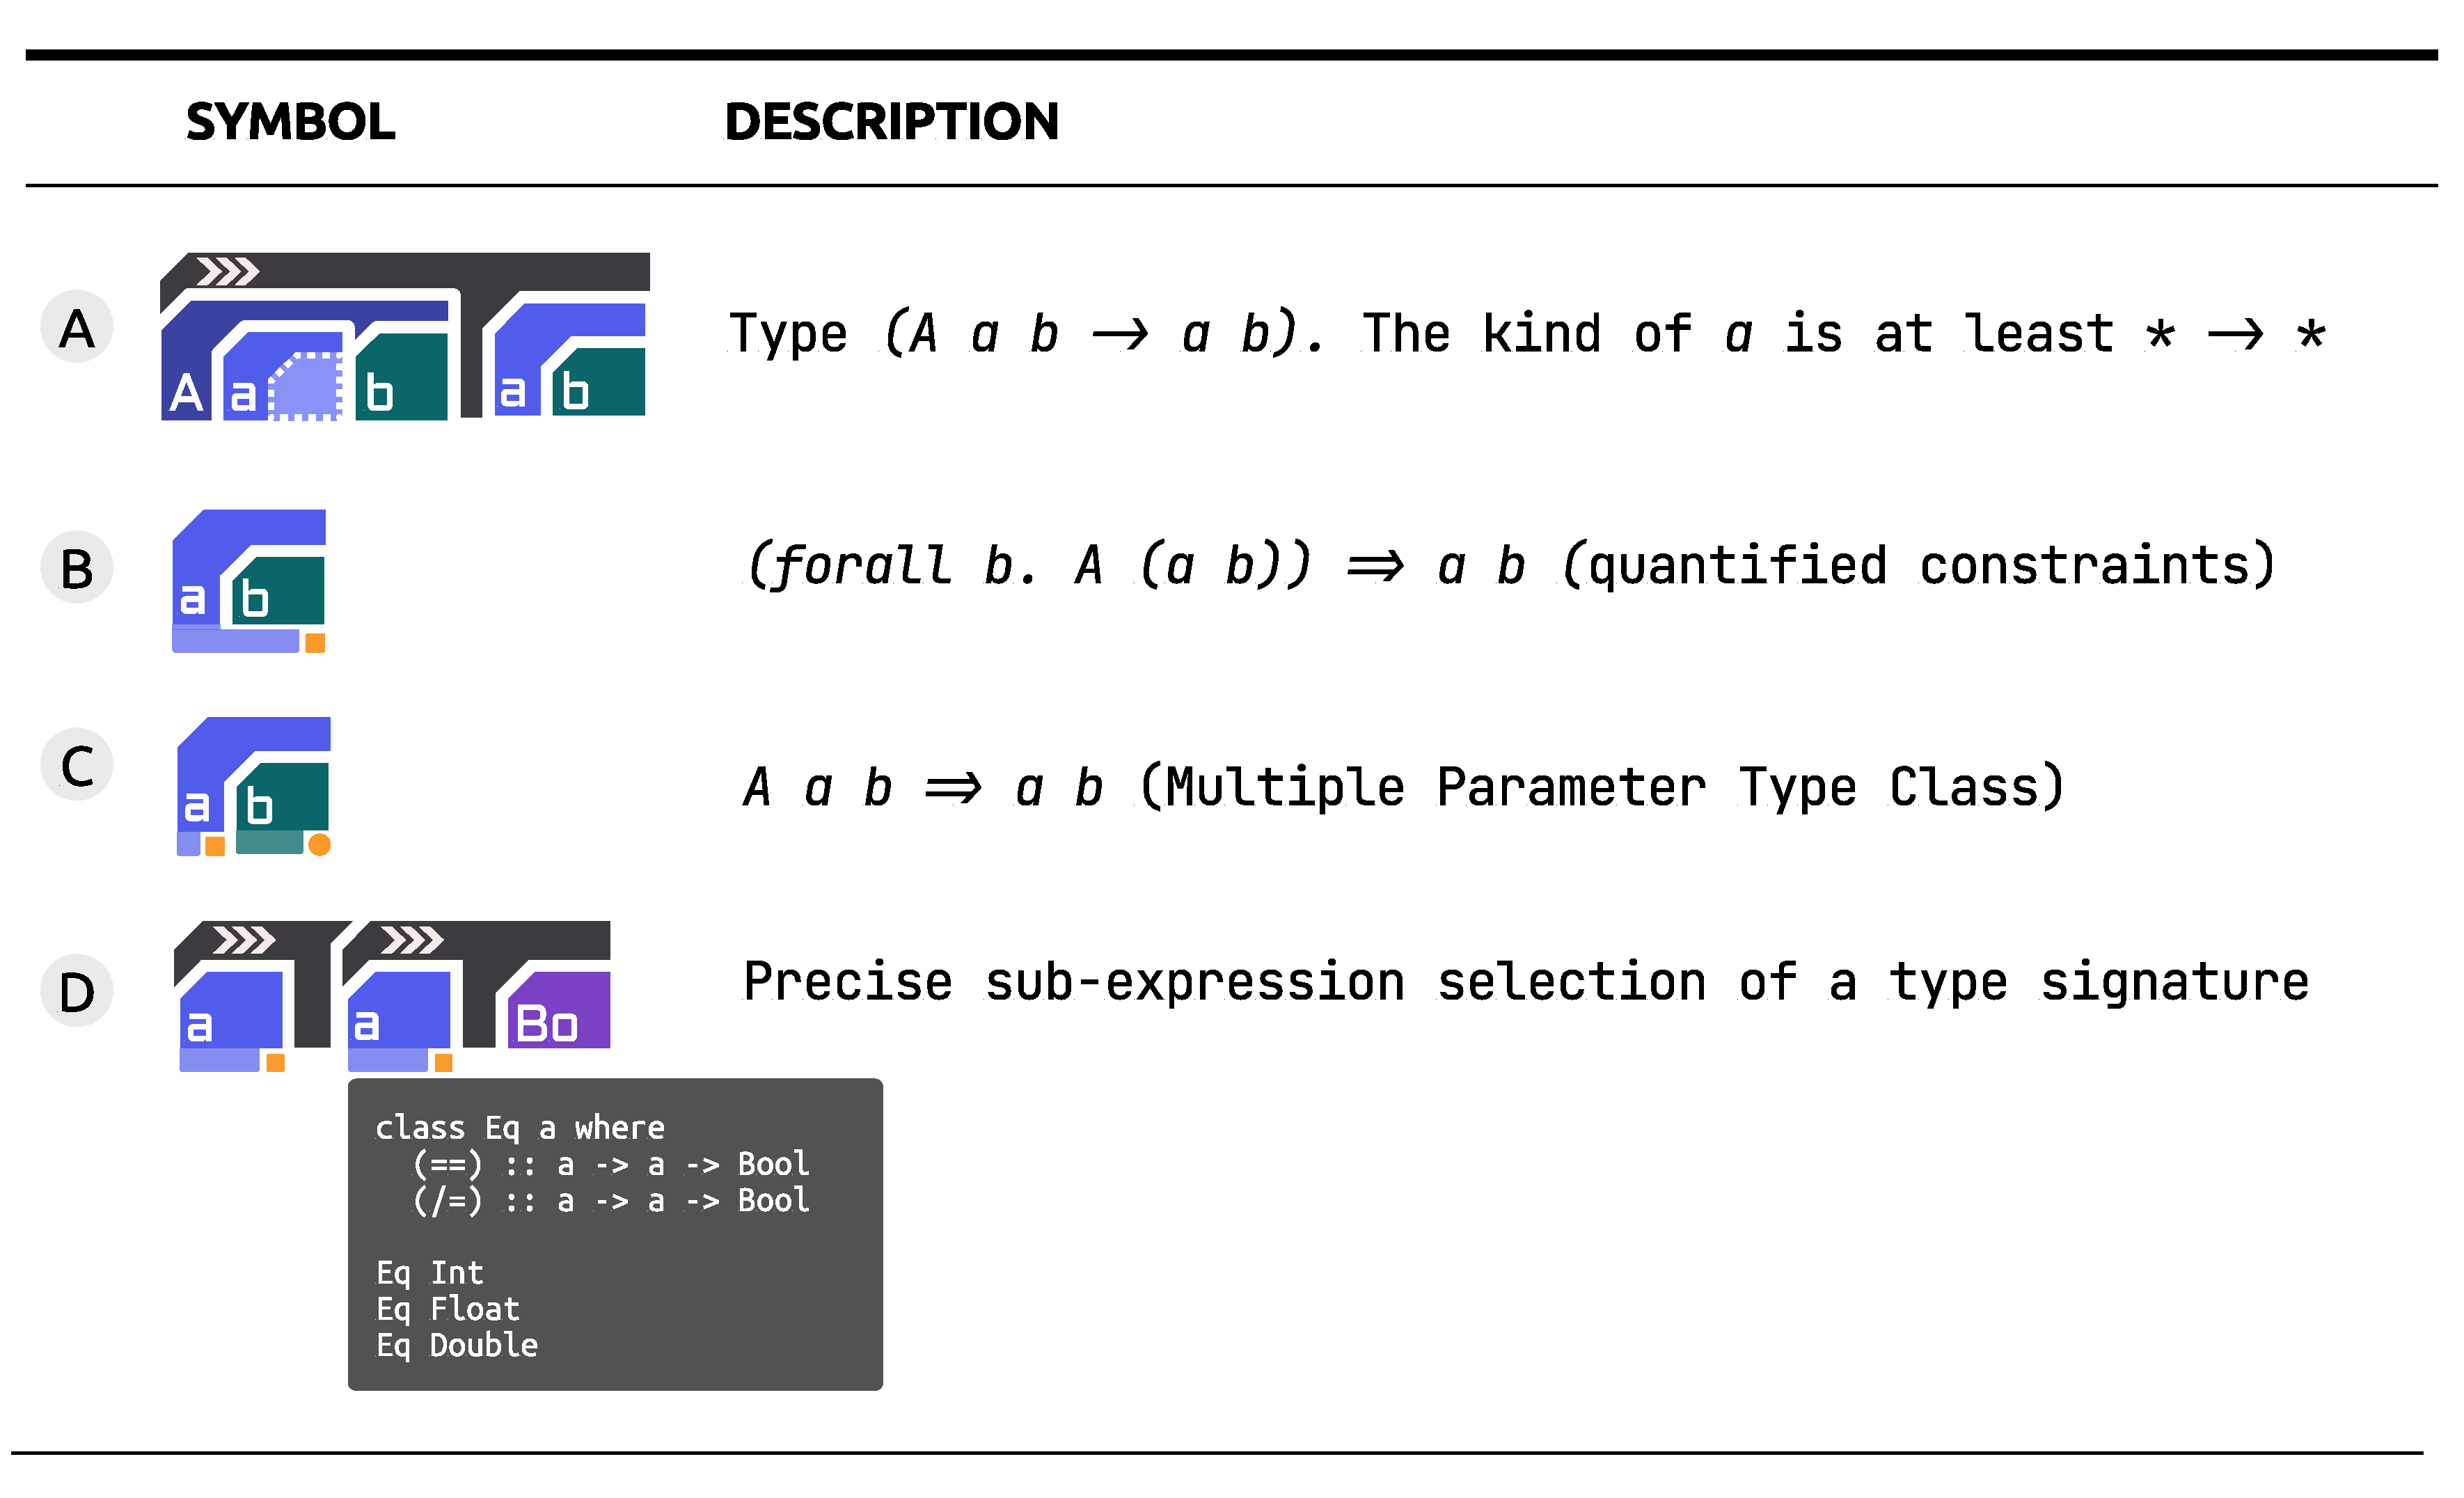
\includegraphics[width=\linewidth]{figures/Advanced}
  \caption{\label{fig:advanced}
  Advanced features of GeckoGraph. (A) Kind visualization. (B)  Qualified constraints. (C)  Multiple Parameter Type Classes. (D) Precise selection of sub-structures. }
\end{figure}


\section{Evaluation} \label{sec:evaluation}
To evaluate the effectiveness of GeckoGraph, we designed and conducted a gamified controlled experiment. The study, ``Zero to Hero", adopted a game-like experience. It contains 10 tasks (levels) of varying difficulty. At each level, participants are asked to implement a function named "\texttt{zeroToHero}" with the help of a limited list of provided functions. These functions are different at each level, and the target types of Zero and Hero vary at each level as well. The details of each level are provided in the Appendix \ref{levels}. 

The experiment aims to study how programmers use and reason about polymorphic types when performing programming tasks. In particular, we studied how programmers scan and select potentially useful functions from a library and how they compare intended types and actual types when type errors are encountered.


\subsection{Example Levels}
\begin{figure}[h]
  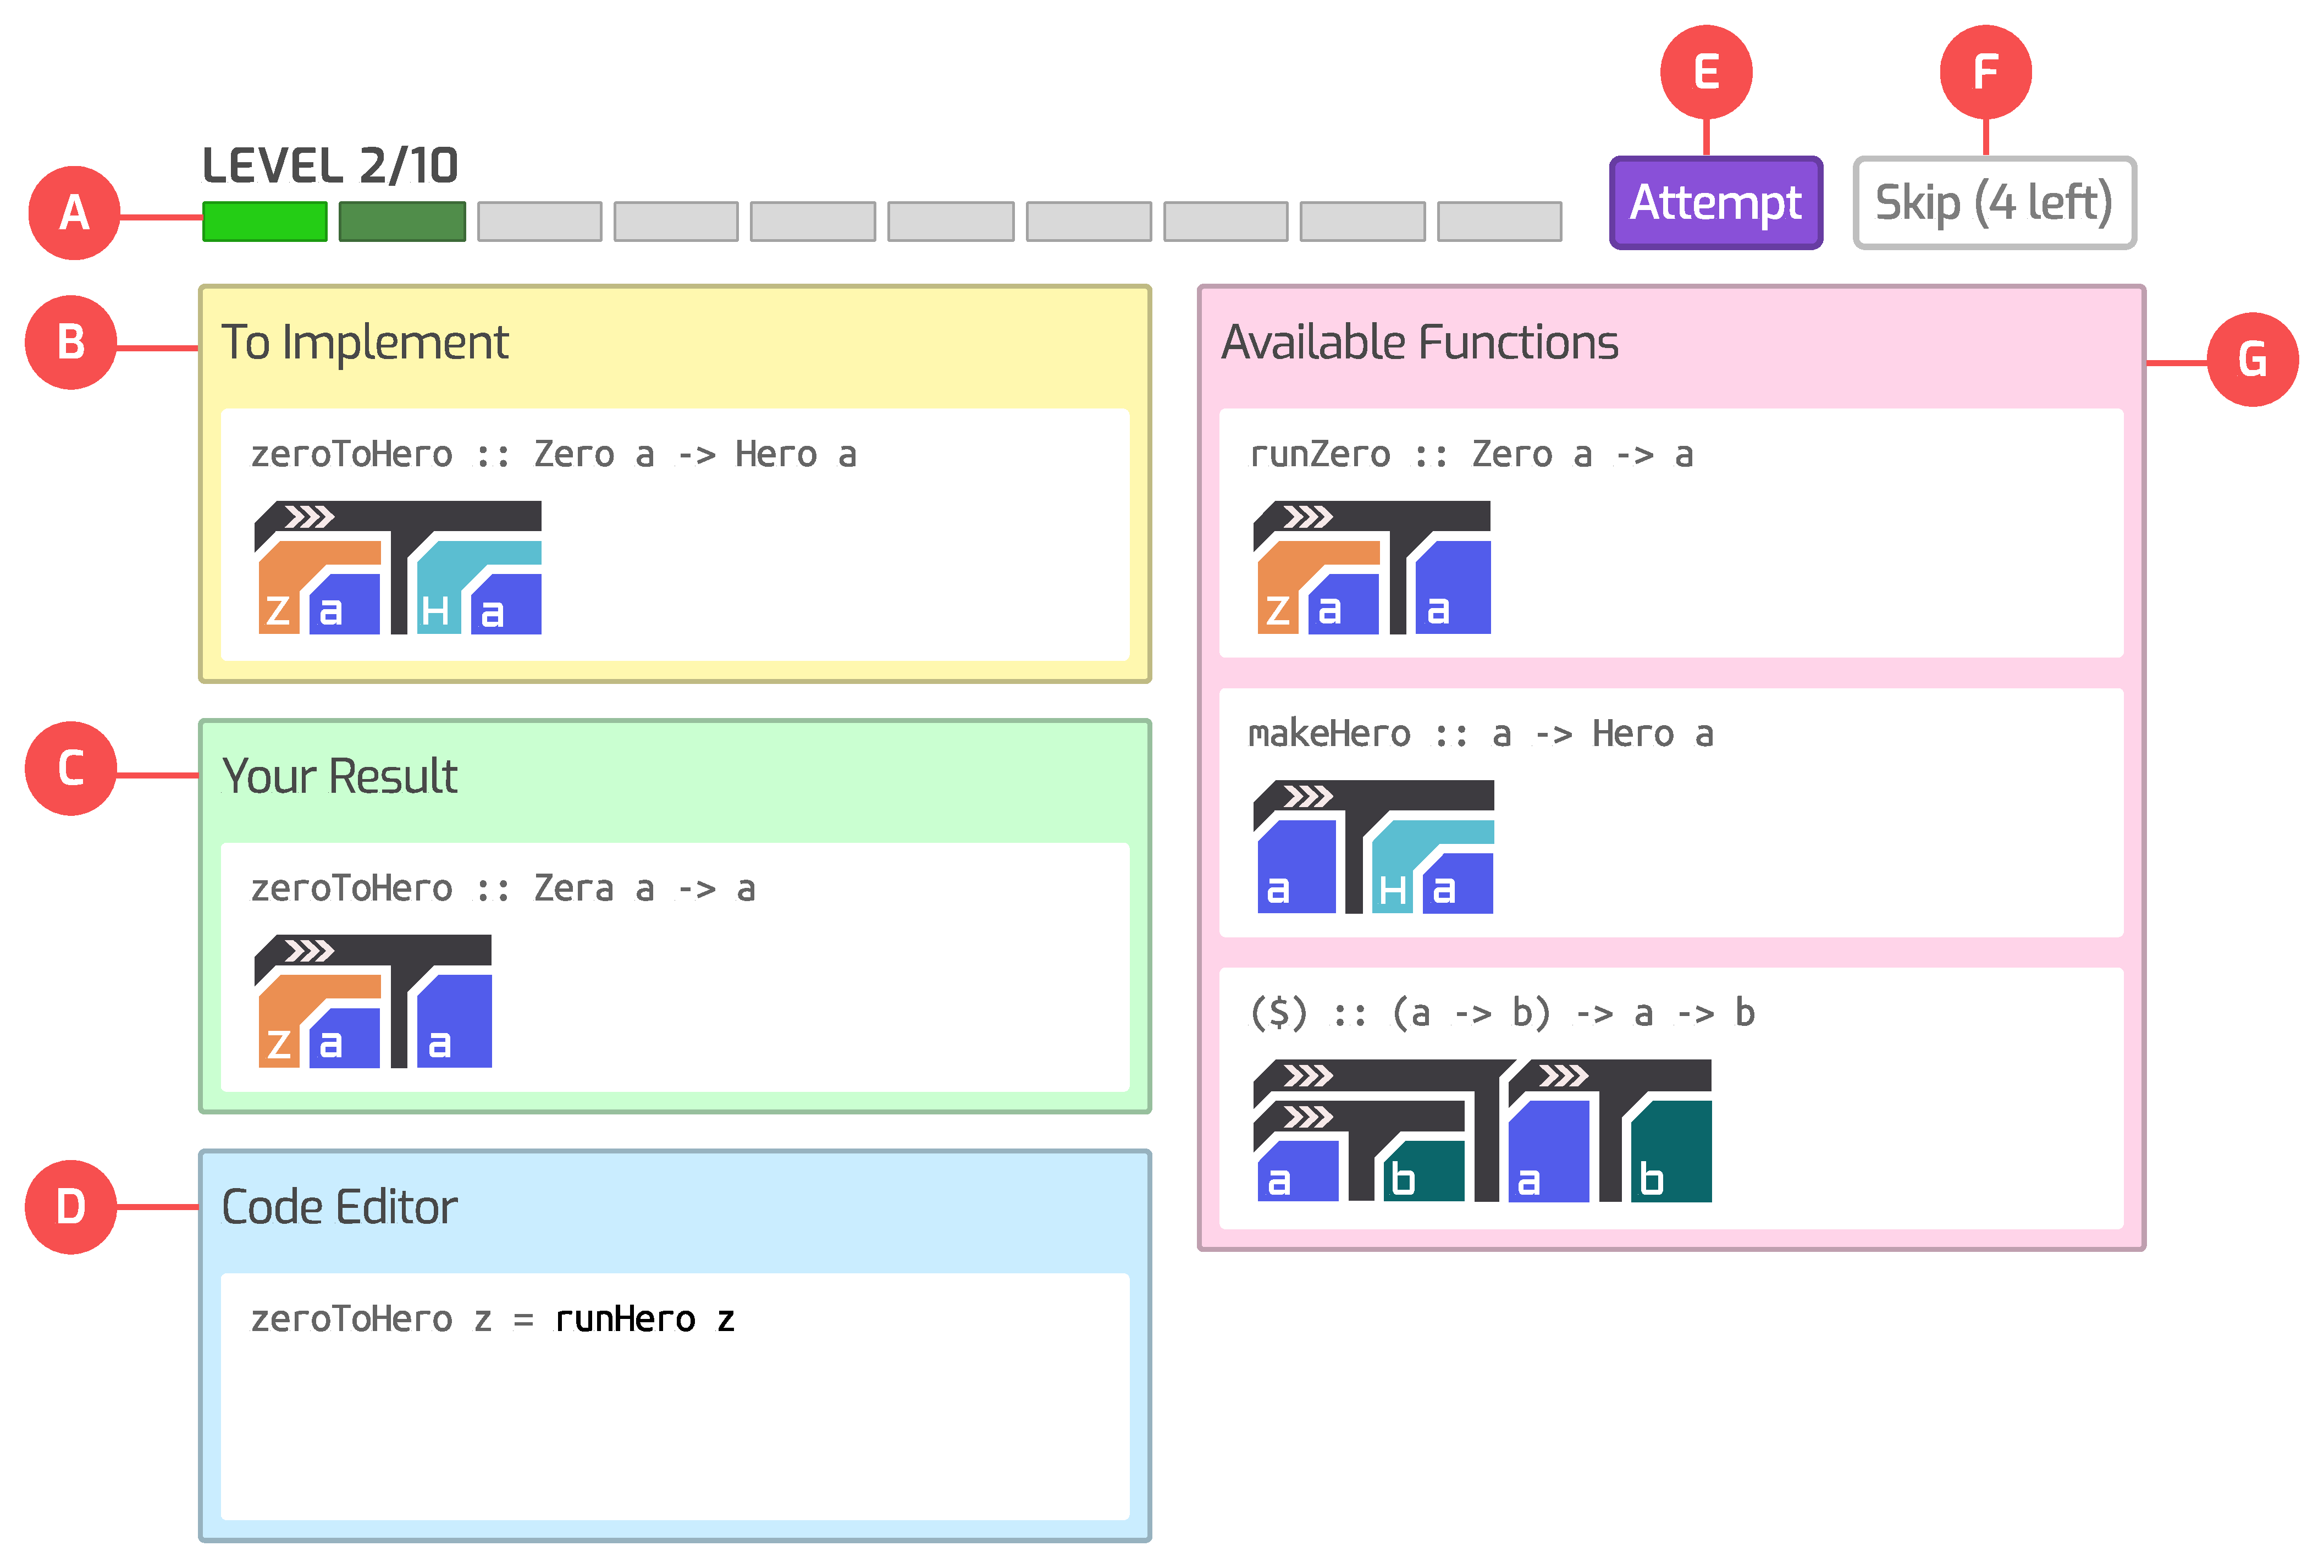
\includegraphics[width=\linewidth]{figures/Level2}
  \caption{\label{fig:level-example} A screenshot from the user study. For this task -- level 2 (Shown at A) -- the players need to implement the function \texttt{ zeroToHero :: Zero a -> Hero a} (B). They write their own definitions in the code editor (D) using a set of provided functions (G). The inferred type of their current definition is shown in (C). When ready, they can test their solution by clicking on the \textit{Attempt} button (E). They can also skip a level by clicking on the \textit{Skip (n left)} button next to it (F).}
  
\end{figure}

We illustrate the tasks of the user study using levels 2 and 3 as examples. For level 2 (Fig. \ref{fig:level-example}), the players need to implement the function \texttt{ zeroToHero :: Zero a -> Hero b}. The available functions are \texttt{runZero::Zero a -> a}, \texttt{makeHero:: a -> Hero a}. A generic function \texttt{(\$)} is provided to improve the ergonomics of composing functions, but all tasks can be completed without the use of generic functions. The possible solutions and other details of the level can be found in Appendix \ref{levels}. To complete this level, players only need to use each of the provided functions once. One possible solution to this task would be {\tt zeroToHero z = makeHero (runZero z)}. The user illustrated in Fig. \ref{fig:level-example} did not reach a correct solution, as the type signature and GeckoGraph in {\it To Implement} panel do not match the one in {\it Your Result} panel.

\begin{figure}[!h]
  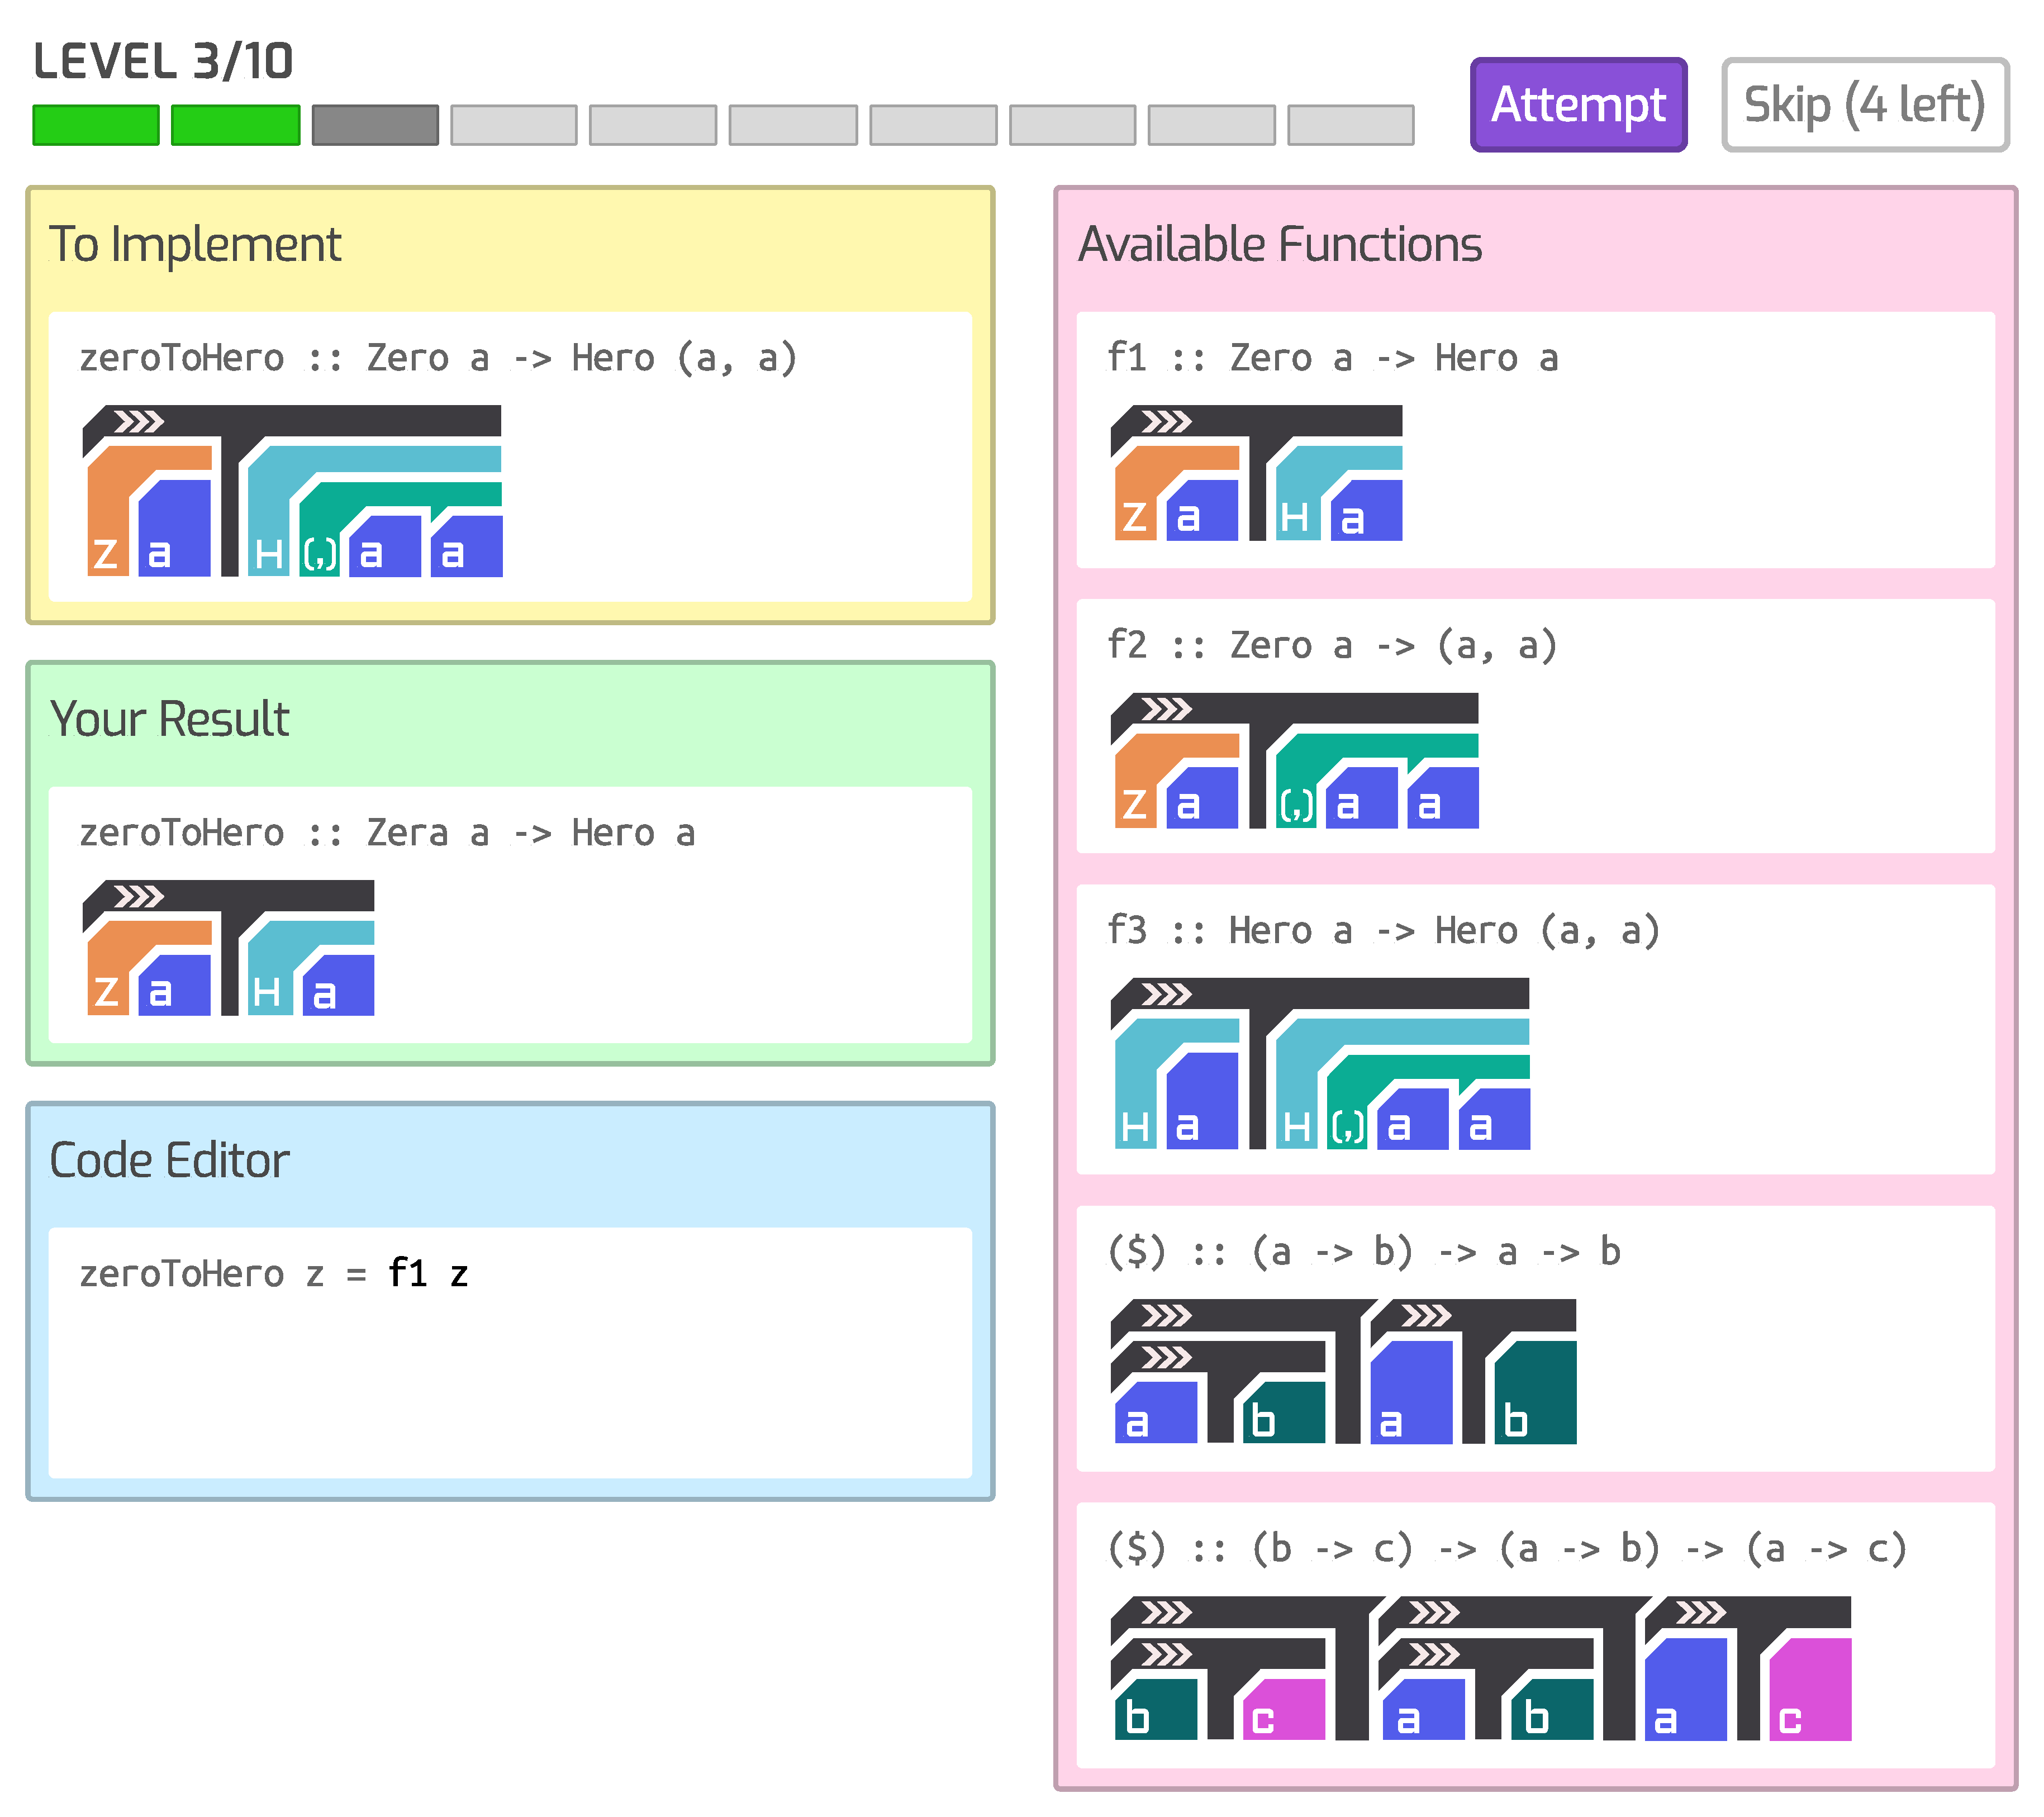
\includegraphics[width=\linewidth]{figures/Level3}
  \caption{\label{fig:level3} A screenshot showing level 3 of the user study.  In this level, the players need to implement the function \texttt{ zeroToHero :: Zero a -> Hero (a a)}. Players are helped by the functions: {\tt f1 :: Zero a -> Hero a}, {\tt f2 :: Zero a -> (a, a)}, and {\tt f3 :: Hero a -> Hero (a, a)}.}
\end{figure}


In level 3 (Fig. \ref{fig:level3}),  players need to implement the function {\tt zeroToHero :: Zero a -> Hero (a, a)}.  In this level, not all provided functions are useful. In particular,  players must discover that only \texttt{f1} and \texttt{f3} are necessary to produce the desired results. One implementation that satisfies the target type is \texttt{zeroTohero z = f3 (f1 z)}. Another possible implementation is {\tt zeroToHero z = f3 . f1 \$ z}, exercising the Haskell function composition idioms. Again, the user illustrated in Fig. \ref{fig:level3} did not reach a correct solution, as the type signature and GeckoGraphs in {\it To Implement} and {\it Your Result} do not match.



\subsection{Recruitment}
Participants were recruited online through the Haskell community on Reddit and Discord. Participation is fully anonymized; detailed ethical implications of these experiments were reviewed and approved by the IRB of the authors' institution.

\subsection{Group Assignments}

Participants are assigned to one of two groups (A and B). The experiment uses a between-subjects design.  The tasks assigned to the two groups are the same. All participants receive both treatments (with and without GeckoGraph) during their runs, but in a different order.   {\bf Group A} is assisted by GeckoGraph on even levels and text-based type annotation on odd levels. {\it Group B} is assisted by text-based type annotation on even levels and GeckoGraph on odd levels. The number of participants in the two groups is counterbalanced.

\subsection{Hypothesis}
In programming tasks that involve reading and understanding polymorphic types, graphic notation using visual elements that provide higher grouping strength (colors, shapes, sizes, and symbols) can improve the performance of such tasks compared to traditional text-based type notation. Our null hypothesis is: {\it Using graphic notation has no effect compared to traditional text-based type notation.} This hypothesis and the task design were registered at the Open Science Foundation prior to data collection \cite{Stuckey2023-vl}. 

\subsection{Task Design} \label{subsection:task}
During the study, participants received 10 tasks. The tasks start off easy but gradually increase in difficulty.  In each task, a target type of the function \texttt{zeroToHero} is shown to the participants. Participants are provided with a list of available functions to implement the target function and to ensure it assumes the target type. This is to simulate the tasks of selecting useful functions from a library. Participants are not allowed to use any other functions or variables outside the provided functions; even the Haskell prelude is not available. This ensures that everyone has the same knowledge and minimizes the effect of familiarity. 

Participants can skip a level if they are stuck. We believe that it is normal for anyone to get stuck on a challenging task, and being stuck on one of the 10 tasks does not discount their feedback on the tool. The number of skips a participant can use is limited to four, so that it is not possible to submit qualitative feedback without completing at least 6 tasks out of 10. 

\subsection{Measurements}
During the study, the time spent by participants on each task is recorded. We also record the resulting status of each level, whether it is a success or a failure. Before starting the study, participants nominate their level of Haskell experience on a four-level scale: beginner, familiar,  knowledgeable, and expert.  If a participant has completed all 10 levels (with the help of skipping), we invite the participant to complete a post-study survey. In it, we ask for them to rate how {\bf intuitive} the GeckoGraph design is, how {\bf distracting} they find GeckoGraph, and how {\bf helpful} GeckoGraph is, using a seven-point scale. In the end, we ask 2 open-ended questions: {\it What is your overall experience using GeckoGraph} and {\it What are your expectations on the potential applications of GeckoGraph}.

Data collection of the study was stopped after the planned cut-off period of 14 days. After the cut-off date, the ZeroToHero website is open-sourced and available for free evaluation\footnote{https://zerotohero.fly.dev}, and repeating our experiment. However, no further data was collected. 

\section{Results}

During the data collection period, a total of 714 users participated in the study. Among them, 245 are novice users, 216 are familiar with Haskell, 216 are knowledgeable users, and 88 are expert users. 

\subsection{Time to complete levels}

The 10 levels are designed to increase difficulty gradually. From the results of the experiment, most of the tasks align with this trend. However, three tasks stand out in Fig. \ref{fig:level-time}.  Level 7 (mean = 334 seconds) is the hardest task in terms of time, followed by level 8 (mean = 228 seconds) and level 5 (mean = 224 seconds). To complete an average level, the beginner group uses an average of 100 seconds, the familiar group uses 90 seconds, the knowledgeable group uses 80 seconds, and the expert group uses 70 seconds. This roughly aligns with self-reported expertise. We show that the task time on each level follows normal distributions using a Shapiro-Wilk test \cite{Shaphiro1965-dx} (p-value  $ \leq 1.018 \times 10^-16$, for an alpha value of 0.05, p less than 0.05 is considered a normal distribution).

Levels 5, 7, and 8 are the only three levels that include functions from the standard Haskell library other than the generic \texttt{(.)} and \texttt{(\$)}, which are provided for pure convenience. Level 5 requires programmers to use the \texttt{fst} and \texttt{snd} functions to extract a value from a tuple. Level 7 requires programmers to use the \texttt{(<*>)} function of the \texttt{Applicative} class, while level 8 requires the \texttt{fmap} function of the \texttt{Functor} class. The authors speculate that the more experienced participants are much more familiar with these functions, hence the strong contrast on these three levels. 

However, when comparing the task time between the two treatments, we were unable to reject the null hypothesis. In a two-sample T-test, we could not find any significant difference between the two groups overall (p-value = 0.457), nor did there differ between the two groups in any of the four levels of experience (beginner: p-value = 0.845, familiar: p-value = 0.524, Knowledgeable: p-value = 0.712, expert: p-value = 0.771).

\begin{figure}[]
  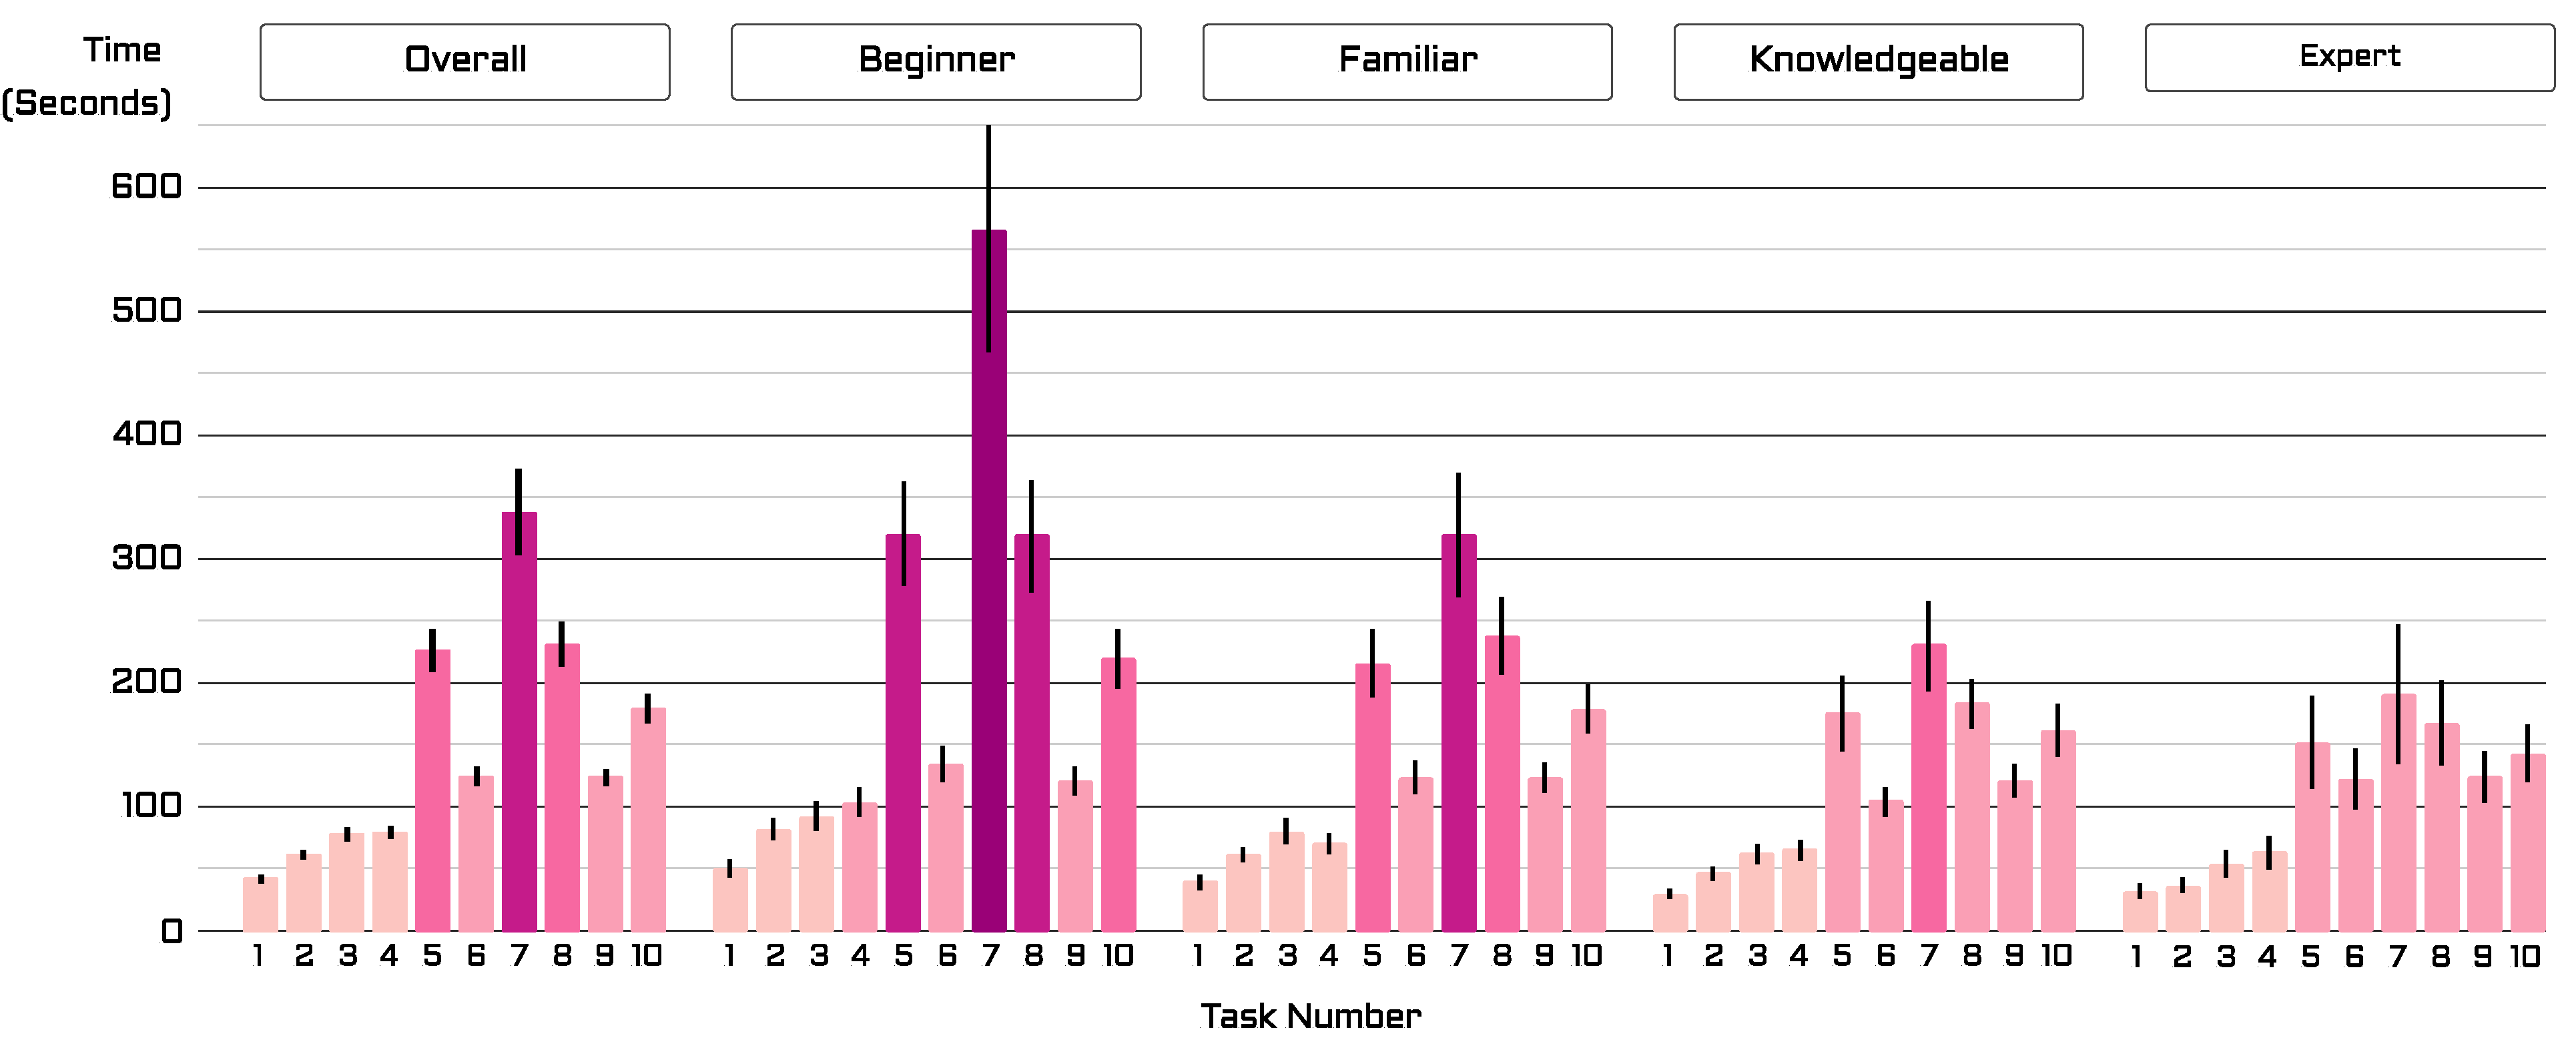
\includegraphics[width=\linewidth]{figures/LevelTime}
  \caption{\label{fig:level-time} Time spent on each level, with 95\% confidence interval. We show that the difficulty steadily increases across the user study, but levels 5, 7, and 8 are significantly harder than the authors intended. The overall task time of each group roughly matches the experience level.}
\end{figure}

\subsection{Success rate}
We saw that, overall, GeckoGraph provides a slightly higher success rate (96.88\%) than text-based type notation (94.62\%). This trend can be seen in every experienced group: beginner group (95.12\% vs. 92.68\%), familiar group (97.39\% vs. 93.34\%), knowledgeable group (96.82\% vs.96.06\%), and expert group (98.2\% vs.96.40\%). We saw the significance decrease as the user's experience increased. When performing a proportion test on each group, we see that the effect is most significant with the beginner group and reject the null hypothesis (z score = 2.0228, p-value = 0.0431), followed by the familiar group (z score = 1.7495, p-value = 0.0802). The knowledgeable group (z score = 1.0295, p-value = 0.3032) and the expert group (z score = 0.8660, p-value = 0.3756) show less significant differences between treatments. 

When breaking down the result in each task (Fig. \ref{fig:success-rate}), we were able to reject the null hypothesis in task 10 of the beginner group (94.9\% with GecoGraph, and 80.4\% without GeckoGraph, p-value=0.0452) and task 10 of the familiar group (98.5\% with GecoGraph, and 87.3\% without GeckoGraph, p-value = 0.136). 

Level 10 is the most cognitively demanding: the provided functions are the lengthiest, and the solution is challenging and deceptive. Programmers must use the provided rotate function {\it f2} to adjust the positions of the four components of the {\it Zero} value four times to get to the correct position. Completing the level requires applying the functions {\it f1}, {\it f2}, and {\it f3} in a nested sequence that is 8 layers deep. Consequently, programmers need to frequently switch contexts to recall the purpose of each function. We speculate that this level demands the mental flexibility typical of a Haskell expert to internalize these functions quickly. GeckoGraph helps less experienced programmers to achieve the same level of comprehension fluency by adding visual clarity.

\begin{figure}[ht]
  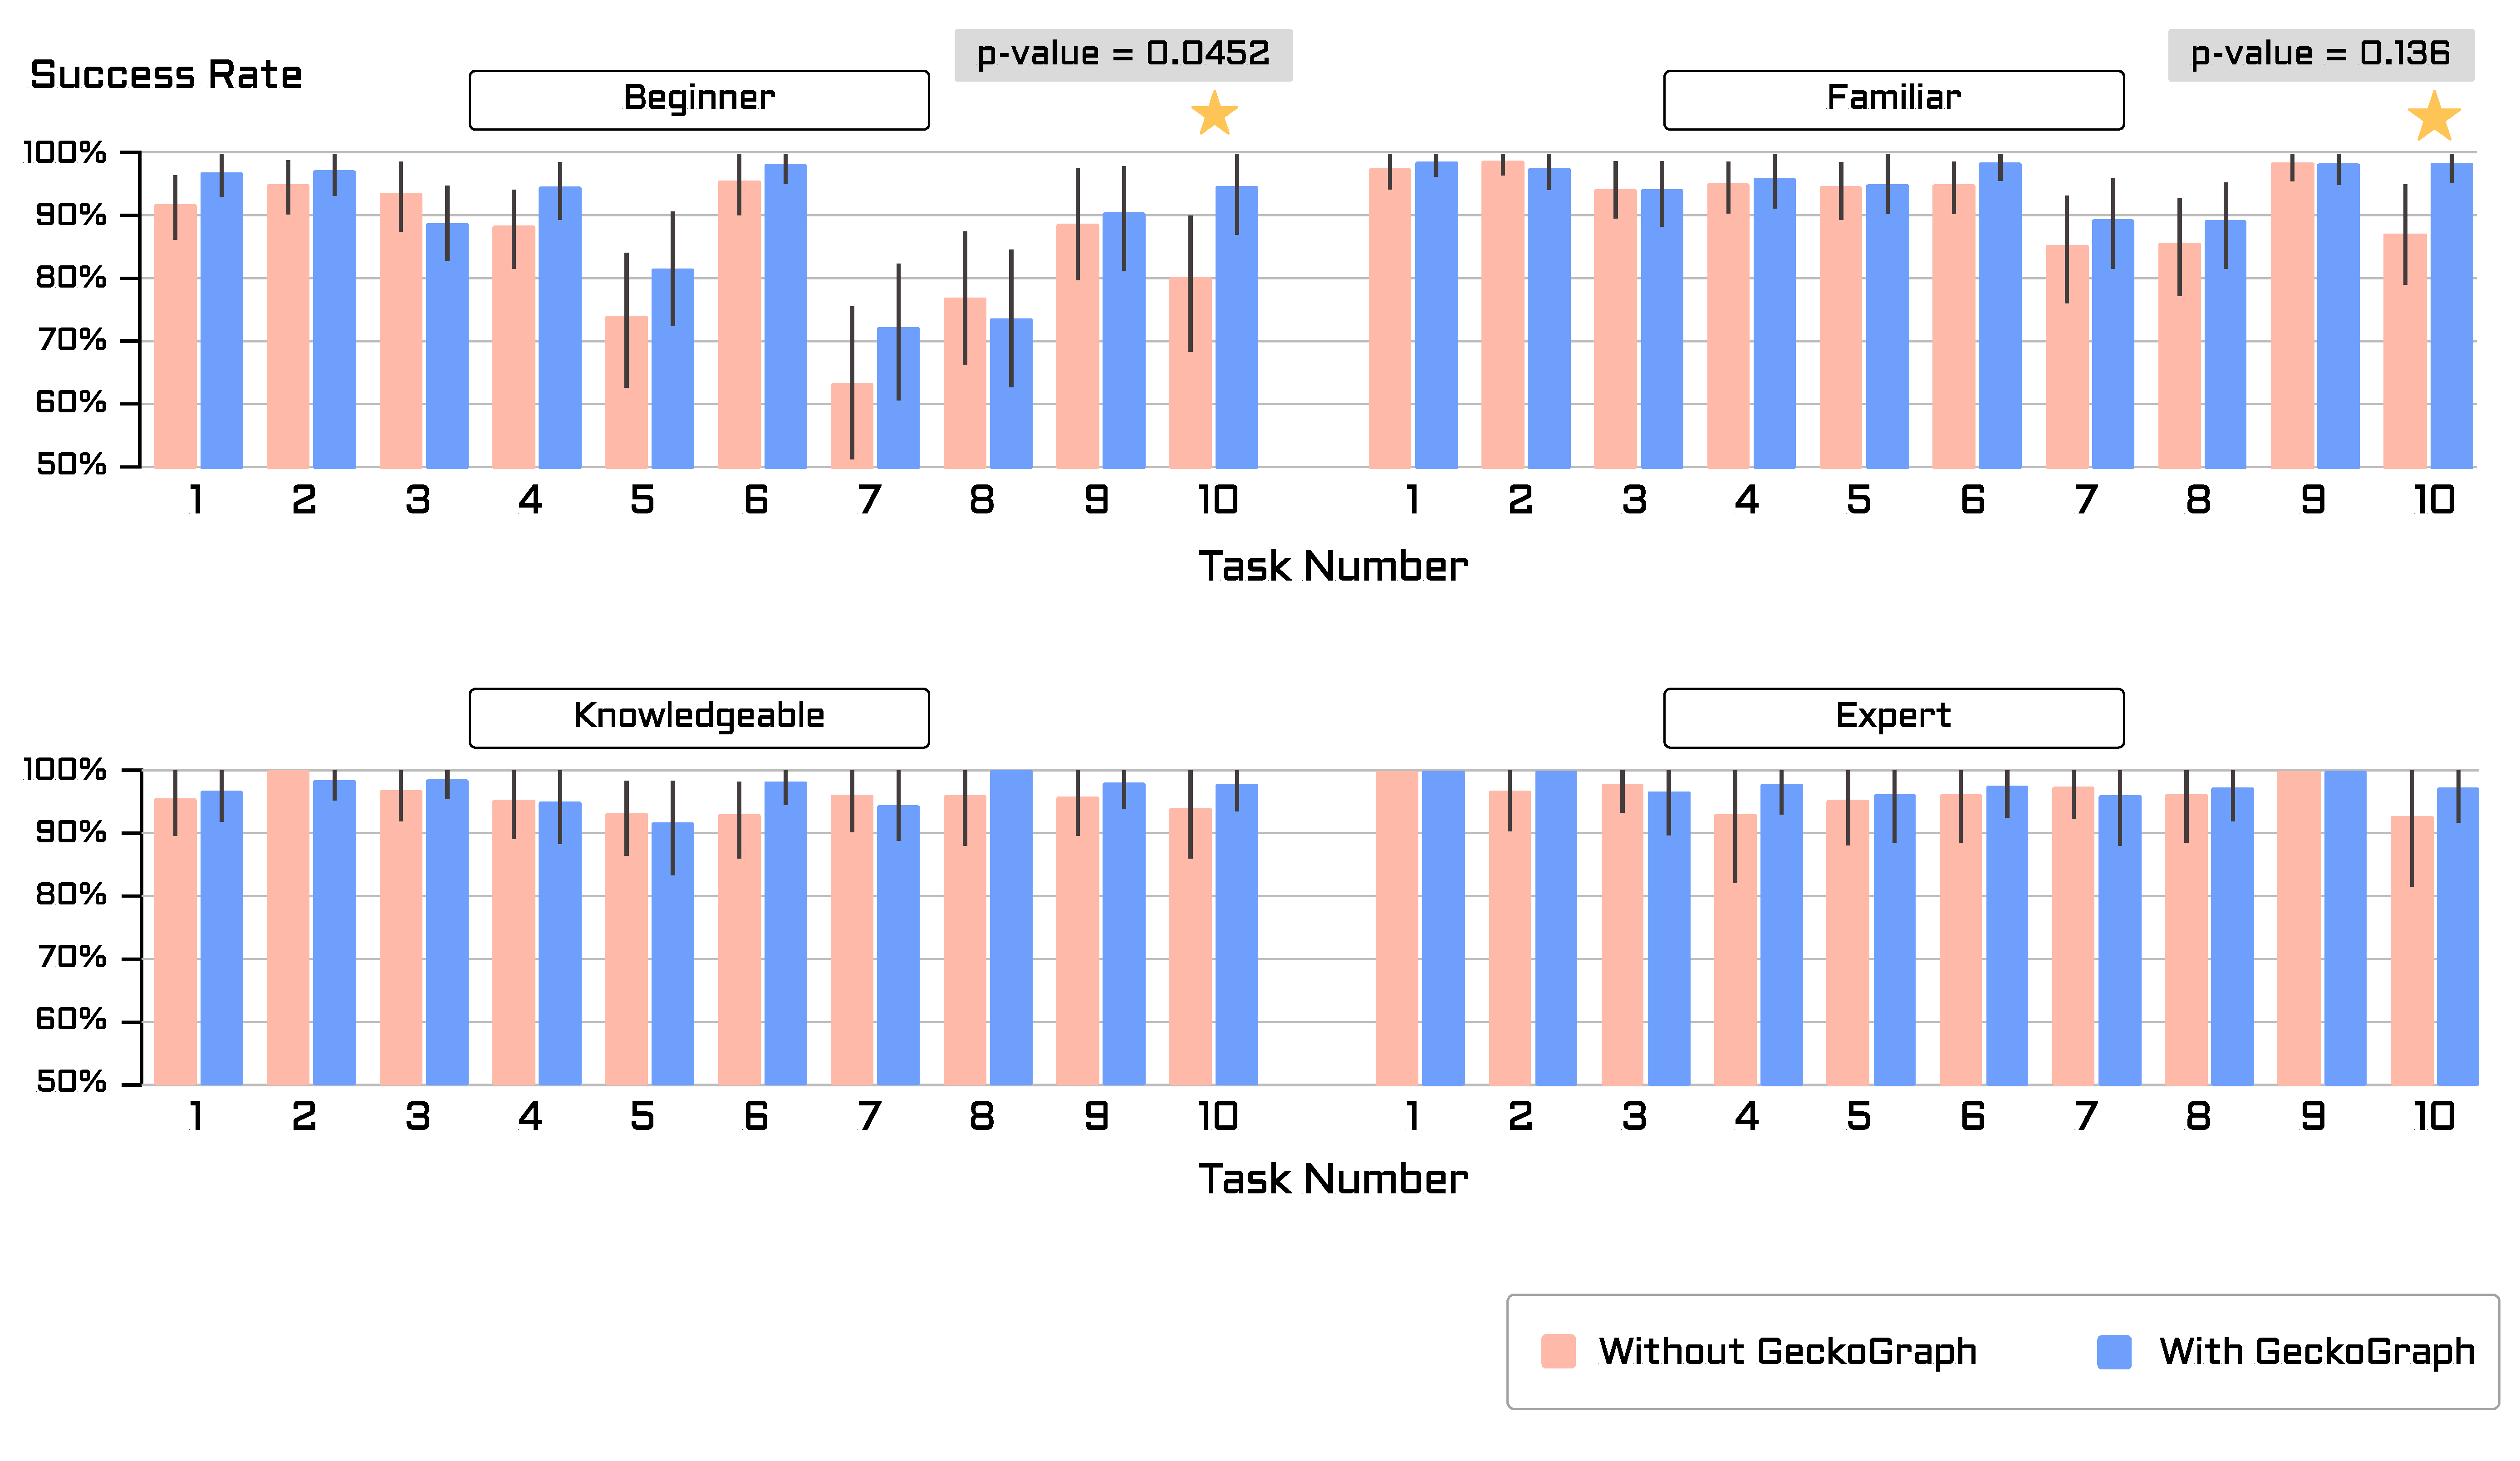
\includegraphics[width=\linewidth]{figures/SuccessfulRate}
  \caption{\label{fig:success-rate}{\bf Success rate of each task, with 95\% confidence interval, grouped by experience level.} The figure is cropped from 50\% to 100\% for readability. Bootstrapping was used for computing the confidence interval because of the non-normal distribution. In most tasks, GeckoGraph provides a small edge. However, significant differences were found in task 10 of the beginner group and task 10 of the familiar group. }
\end{figure}

\subsection{Qualitative Feedback}
In their responses to the post-study survey, participants showed mostly neutral sentiments towards GeckoGraph's design and appeal. They find GeckoGraph moderately intuitive to use and that its appearance in the interface does not cause distraction.

For the question ``Do you find the GeckoGraph distracting", most of the participants rated a low score, with an average of 2.88 (Fig. \ref{fig:qualitative} left). For the question ``How intuitive do you find the GeckoGraph?", we saw a reverse correlation of experience (Fig. \ref{fig:qualitative} Middle): experts find the GeckoGraph most intuitive (5.07), followed by the knowledgeable group (4.87), and the familiar group (4.80). The beginner group found it to be the least intuitive but still rated it positively, albeit with a low score of 4.71. 
When answering the question ``How helpful do you find GeckoGraph in finding the solution?", the answer is more divided into different experience groups (Fig. \ref{fig:qualitative} right). It is slightly positive for beginners (mean=4.25) and slightly negative for the other groups, the familiar group (mean=3.86) and the knowledgeable group (mean=3.32). The expert group finds that GeckoGraph is moderately unhelpful (mean=2.95)

Two interesting trends emerge. First, experienced users are more likely to find GeckoGraph intuitive and easy to use. This aligns with our design decision to make GeckoGraph resemble text-based type annotation. Those familiar with text-based type annotation find GeckoGraph second nature to read. Second, the correlation reverses when it comes to perceived helpfulness. The more experienced the users are, the less likely they are to find GeckoGraph helpful. We speculate this pattern occurs because users who are experts in text-based type annotations naturally prefer reading text-based notation and tend to ignore GeckoGraph, diminishing its usefulness. Conversely, novice users are more likely to be drawn to GeckoGraph and find that its visualization offers more clarity and useful insights.


% To quote some feedback from participants: ``Types are much easier to understand by the GeckoGraph than by trying to parse all parentheses and understand the types from the signature. " ``It makes it easier to see at a glance when your output type is correct or what the difference between the current type and the target is."

% To quote a participant, ``GeckoGraph is quite intuitive to see the permutations of the arguments. Also, to see how to produce and consume arguments." 

\begin{figure}[]
  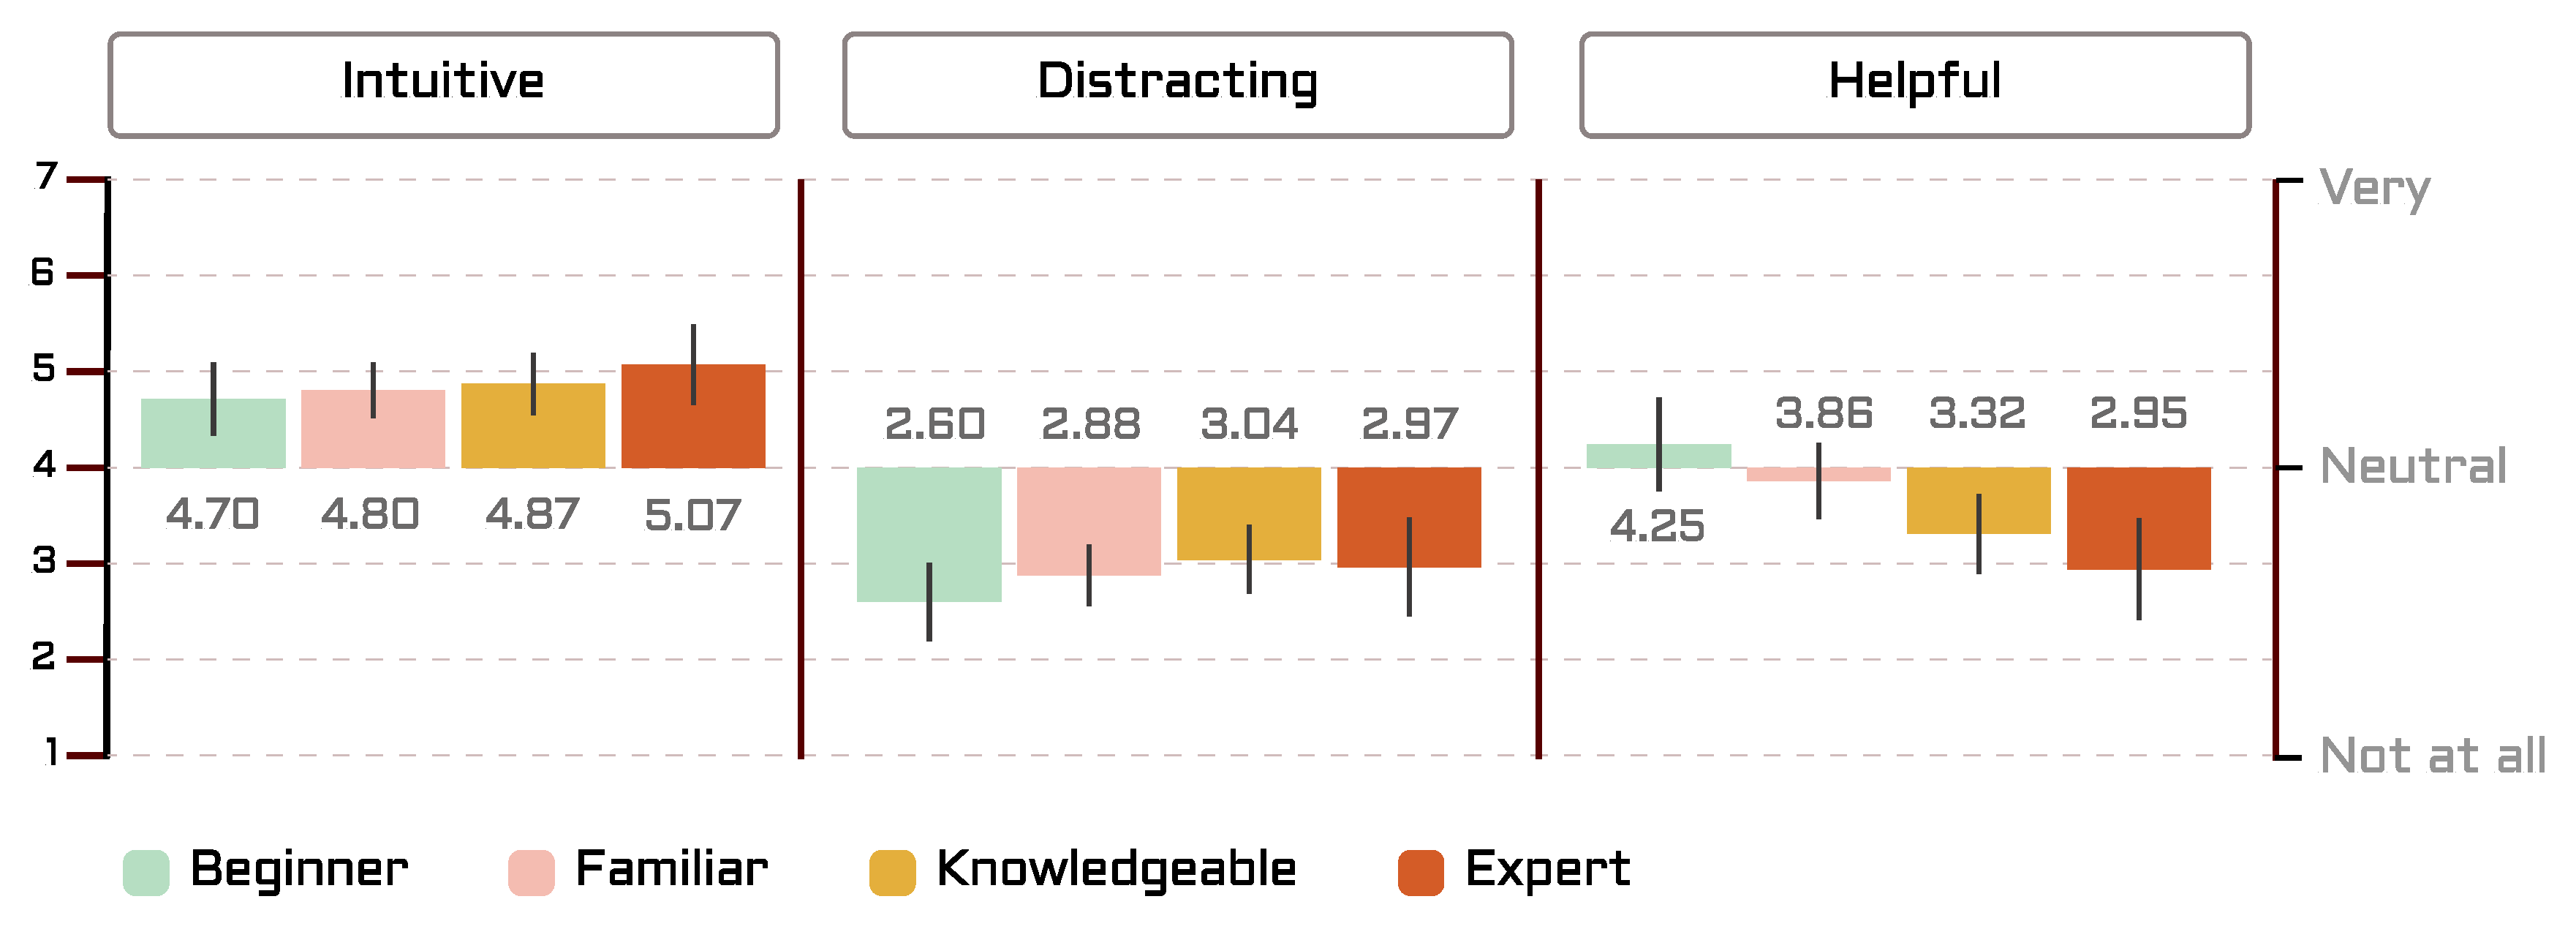
\includegraphics[width=\linewidth]{figures/Qualitative}
  \caption{\label{fig:qualitative} {\bf The users rated scores of how intuitive (left), distracting (middle), and helpful (right) they found GeckoGraph, with 95\% confidence interval.} Overall, programmers are neutral to GeckoGraph's design. Some find GeckoGraph to be intuitive and not distracting. However, beginners are more likely than experienced functional programmers to find it helpful. }
\end{figure}

\subsection{Threats to validity}

\paragraph{Task design}
In our user study, most of the provided functions are very abstract. These functions are created by the authors solely for the gamified study. They are designed to be different from well-known Haskell functions to minimize the familiarity variable. They are also designed with an interest in being challenging and fun. These functions may not be the most representative of real-world Haskell programming. 

\paragraph{The use of skips}
Although we justified the use of skips in Section \ref{subsection:task}, the availability of skipping does allow users to adopt more utilitarian strategies, often involving skipping a level without giving it a fair try. This happened more often in the later levels when users realized they had enough skip opportunities left to ``complete the game". These strategies may result in lower recorded success rates than if no skips were allowed.


\section{Discussion} \label{sec:discussion}

This section discusses the main findings and implications of our study. 
We begin by outlining the strengths of GeckoGraph observed from both quantitative and qualitative results (Section~\ref{sec:discussion:strengths}). 
We then discuss the limitations of the current design (Section~\ref{sec:discussion:weaknesses}) and reflect on the gamified nature of our user study (Section~\ref{sec:discussion:gamification}). 
Finally, we identify potential applications of GeckoGraph in programming tools, documentation, and education (Section~\ref{sec:discussion:applications}).

\subsection{Strengths}\label{sec:discussion:strengths}
Overall, our experimental results show no statistically significant difference in task completion time between conditions with and without GeckoGraph. However, we find that using GeckoGraph shows a significant albeit moderate effect on the task success rates for beginners. Particularly, in the hardest task (task 10), GeckoGraph improved the success rates across the two less experienced user groups by 14.5\% and 11.2\%, respectively. 
To interpret the observed advantages, we discuss the practical benefits that GeckoGraph offers to programmers.

\subsubsection{Identifying the Most Important Features}
Qualitative feedback revealed that programmers found GeckoGraph particularly helpful for spotting patterns and identifying important features in type signatures. 
Participants appreciated how GeckoGraph highlights key aspects of a type using distinctive visual properties such as color, length, and height. 
Representative comments include: 
``{\it Types are much easier to understand with GeckoGraph than by trying to parse all parentheses and understand the types from the signature.}'' and 
``{\it It makes it easier to see at a glance when your output type is correct or what the difference between the current type and the target is.}''

\subsubsection{Generalizing Patterns in Type Classes}
A common source of confusion among novice Haskell programmers is distinguishing between functions that operate on generic types and those that work on concrete types \cite{Tirronen2015-nr}. 
For example, differentiating between {\tt Integral a => a} and {\tt Integer}, {\tt Floating a => a} and {\tt Float}, or {\tt Foldable} and {\tt []} can be difficult. 
Learners often find such distinctions irrelevant to their immediate tasks, which complicates problem-solving and error interpretation.

As shown in Fig.~\ref{fig:example-foldable}, when a programmer mistakenly supplies a \texttt{Char} instead of a \texttt{String}, the compiler reports a confusing mismatch involving a generalized type \texttt{t0 a0}. 
In GeckoGraph, both list types and types with a \texttt{Foldable} instance share similar visual structures. 
This correspondence helps programmers relate generalized types back to familiar concrete ones, lowering the cognitive barrier to understanding polymorphism. 
Such visual consistency is especially valuable in Haskell, where even simple arithmetic operators like {\tt +} and {\tt -} are defined generically.

\subsubsection{Consistent Color Scheme}\label{par:color-scheme}
A frequent task in programming is scanning through documentation or libraries to find a desired function, often based on partial knowledge such as argument types, arity, or expected output. 
For example, one might look for a conversion from \texttt{String} to \texttt{Data.Text}, or a function like \texttt{lookup} that operates on \texttt{Data.Map a b} and returns a value of type \texttt{b}. 
GeckoGraph supports this by assigning consistent colors to identical type identifiers, allowing programmers to visually group related types and quickly locate relevant functions.

\subsubsection{Low Barrier to Learning and Understanding}
GeckoGraph retains key conventions from traditional textual type notation: it follows left-to-right reading order, preserves symbolic names as secondary encodings, and mimics prefix and infix structures. 
These design choices ensure that programmers familiar with Haskell can intuitively understand and use GeckoGraph with minimal training.

This ease of adoption was evident in user feedback. Several participants noted that they had no prior Haskell experience but were able to solve the puzzles successfully with GeckoGraph’s help. 
Comments included: 
``{\it It is similar enough to traditional types that it feels intuitive.}'' and 
``{\it This was how I parse the textual representation of types.}''

\subsubsection{Language Agnostic}
GeckoGraph can be implemented in any statically typed language. 
This makes it useful in multi-language programming environments—such as projects combining client-server architectures or foreign function interfaces—where it can provide a unified visual notation across different syntaxes. 
In education, GeckoGraph abstracts away naming differences between languages. 
For example, the product type in algebraic data types is known variously as a \textit{record}, \textit{struct}, or \textit{named tuple}. 
GeckoGraph helps unify these equivalent concepts visually, promoting language-independent understanding.

\subsection{Weaknesses}\label{sec:discussion:weaknesses}
\subsubsection{Space Usage}\label{subsec:space}
GeckoGraph’s layout scales horizontally with the size of a type’s syntax tree and vertically with its depth. 
Compared to traditional text-based notation, this results in higher vertical space consumption. 
We have identified possible optimizations, such as displaying only color blocks while omitting textual identifiers, to reduce space usage while preserving the main advantages of the design.

\subsubsection{Color Encoding}
GeckoGraph relies heavily on color as its primary visual channel. 
While this offers strong perceptual grouping \cite{Zeng2023-jz}, color perception varies among individuals, posing accessibility challenges for visually impaired programmers. 
Although GeckoGraph adopts color-blind–friendly palettes, this only mitigates some issues. 
To improve accessibility, future work will explore alternative encodings such as patterns and shapes in addition to color.

\subsection{Gamified Human Study}\label{sec:discussion:gamification}
Our user study was intentionally designed as a game-like experience, incorporating multiple gamification techniques such as levels, story elements, and goals/rewards \cite{Hamari2014-mc}. 
This approach ensured participant motivation and contributed to a historically high participation rate within the Haskell community. 
Gamification has been widely shown to enhance engagement and motivation in human–computer interaction research \cite{He2014-vp}. 
In our context, it helped attract a diverse set of participants across a wide range of experience levels, addressing a common challenge in studies of functional programming.

\subsection{Potential Applications}\label{sec:discussion:applications}

\subsubsection{Programming Assistance}
Post-study feedback highlighted a strong interest in integrating GeckoGraph into programming environments. 
Modern IDEs already allow users to inspect expression types via hover tooltips; GeckoGraph could enhance this feature by visualizing type structures directly in the tooltip. 
Similarly, GeckoGraph could be used to visualize mismatched parts of conflicting types during compilation errors, as illustrated in Fig.~\ref{fig:example-foldable}.

\subsubsection{Documentation Assistance}
Our findings suggest GeckoGraph would be highly effective for visualizing function types in API documentation and programming libraries. 
Because GeckoGraph representations can be generated automatically, integration into documentation systems like Hoogle \cite{Mitchell_undated-fb} would require minimal effort. 
A quick visual scan of the page can quickly review the theme of a library or package, i.e., the domains and codomains most functions operate on. For instance, a library that mostly supports string operations should predominantly show the color of {\tt String} type, while a low-level graphics-related library may show mainly the colors for {\tt Vector} type and {\tt Float} type.

\subsubsection{Pedagogical Applications}
GeckoGraph can serve as a valuable teaching aid for introducing programming language concepts that are abstract or difficult to explain textually. 
Several study participants with no prior Haskell experience reported that GeckoGraph helped them understand type-related puzzles and complete all tasks successfully. 

Beyond basic learning, GeckoGraph’s advanced features (Section~\ref{sec:benefits}) also make it suitable for teaching higher-level functional programming concepts. 
For instance, consider the \texttt{assoc} function for day convolution \cite{Day1970-kb} in the Kan extension (Fig.~\ref{fig:assoc}). 
Although the type signature is concise, it is cognitively difficult to parse due to multiple variables and their hidden kinds. 
GeckoGraph reveals these higher-kinded types visually, exposing partially applied data types and making the semantics easier to understand.

\begin{figure}[]
  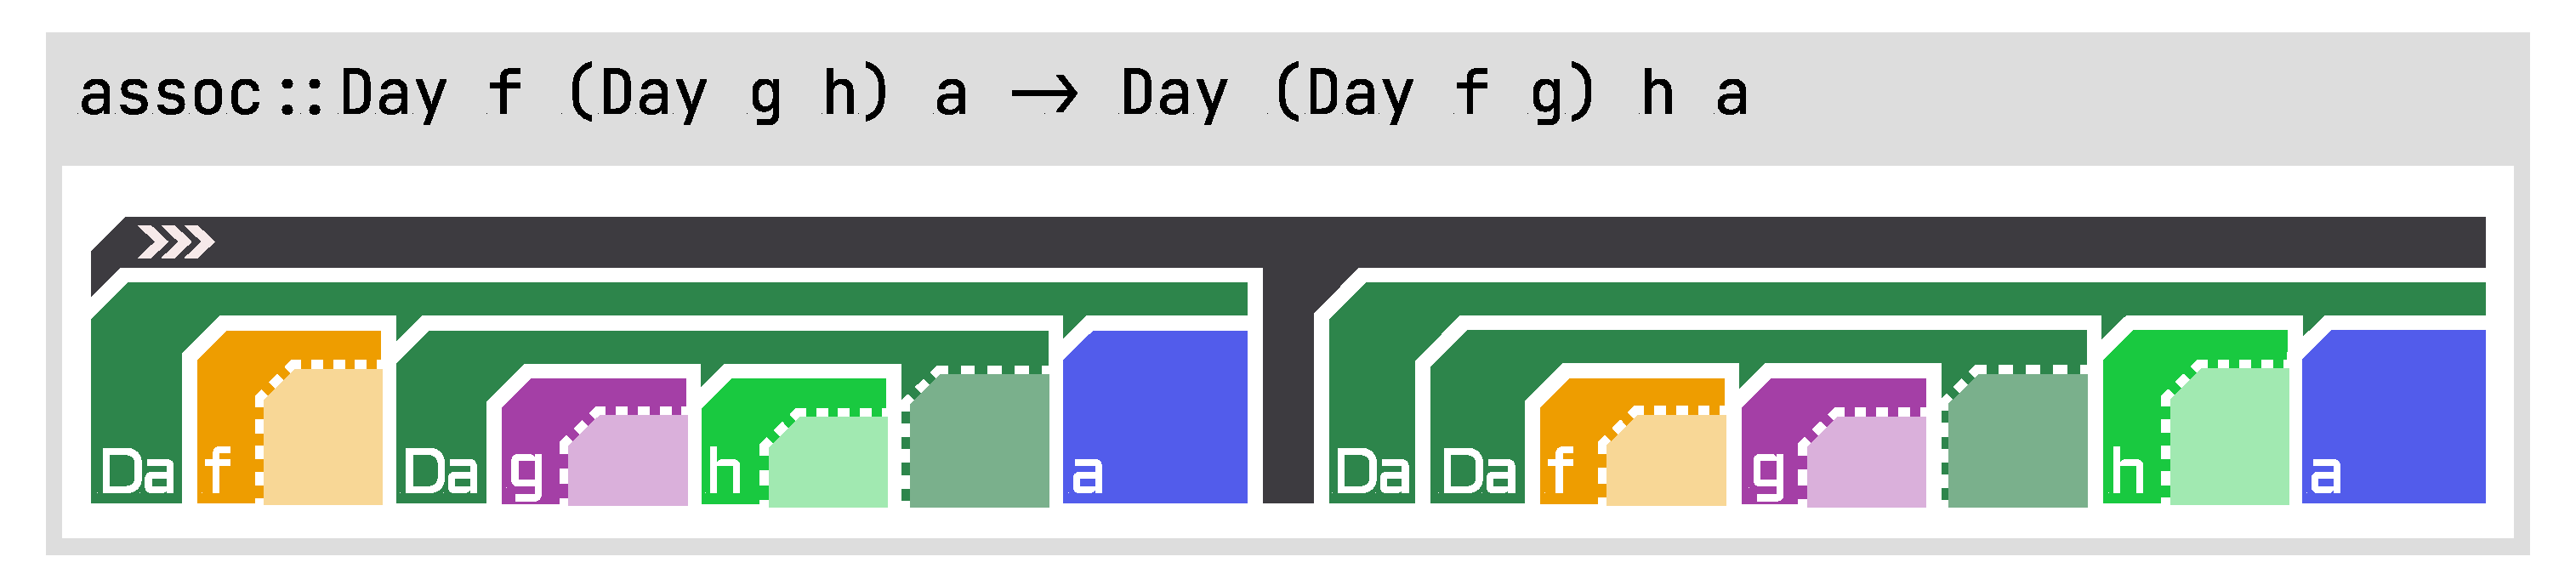
\includegraphics[width=\linewidth]{figures/assoc}
  \caption{\label{fig:assoc} 
  The \texttt{assoc} function for day convolution \cite{Day1970-kb} in the Kan extension. 
  Even without knowing the exact definitions, viewers can easily see that \texttt{f}, \texttt{g}, and \texttt{h} are all higher-kinded types—information that is obscured in traditional textual notation.}
\end{figure}


\section{Related work}
This section reviews prior work in three areas relevant to this research. First, we examine approaches to the visualization of types in programming languages. 
We then broaden our view to general visualization techniques applied to programming environments, including topics like memory allocation and change history. Finally, we review studies comparing visual and textual representations in programming education and environments.

\subsection{Visualization of Types}
A similar half-enclosing structure was proposed in Jung’s visualization of types~\cite{Jung2000-oc}. In Jung’s notation, the type constructor partially encloses its arguments, but its figure is positioned at the bottom right (Fig.~\ref{fig:jung}). In contrast, GeckoGraph follows a natural left-to-right reading order, allowing larger structures in a type signature to take visual precedence over smaller ones. 

Compared to Jung’s approach, GeckoGraph offers two major advantages. 
First, it naturally represents the general notion of a curried function. Partial application can be intuitively read as removing the first argument, which is not as clear in Jung’s notation. 
Second, the shape of a function type remains visually consistent with that of normal data types. In Jung’s design, a function type such as \texttt{a -> b} looks markedly different from a data type \texttt{f a b}. 
This distinction is important because, in functional languages, abstractions often generalize over both functions and data types. 
For example, both functions and lists have \texttt{Functor} instances, allowing their inner values to be transformed using \texttt{fmap}. 
GeckoGraph’s consistent visual shape helps make such generalizations more apparent.

\begin{figure}
  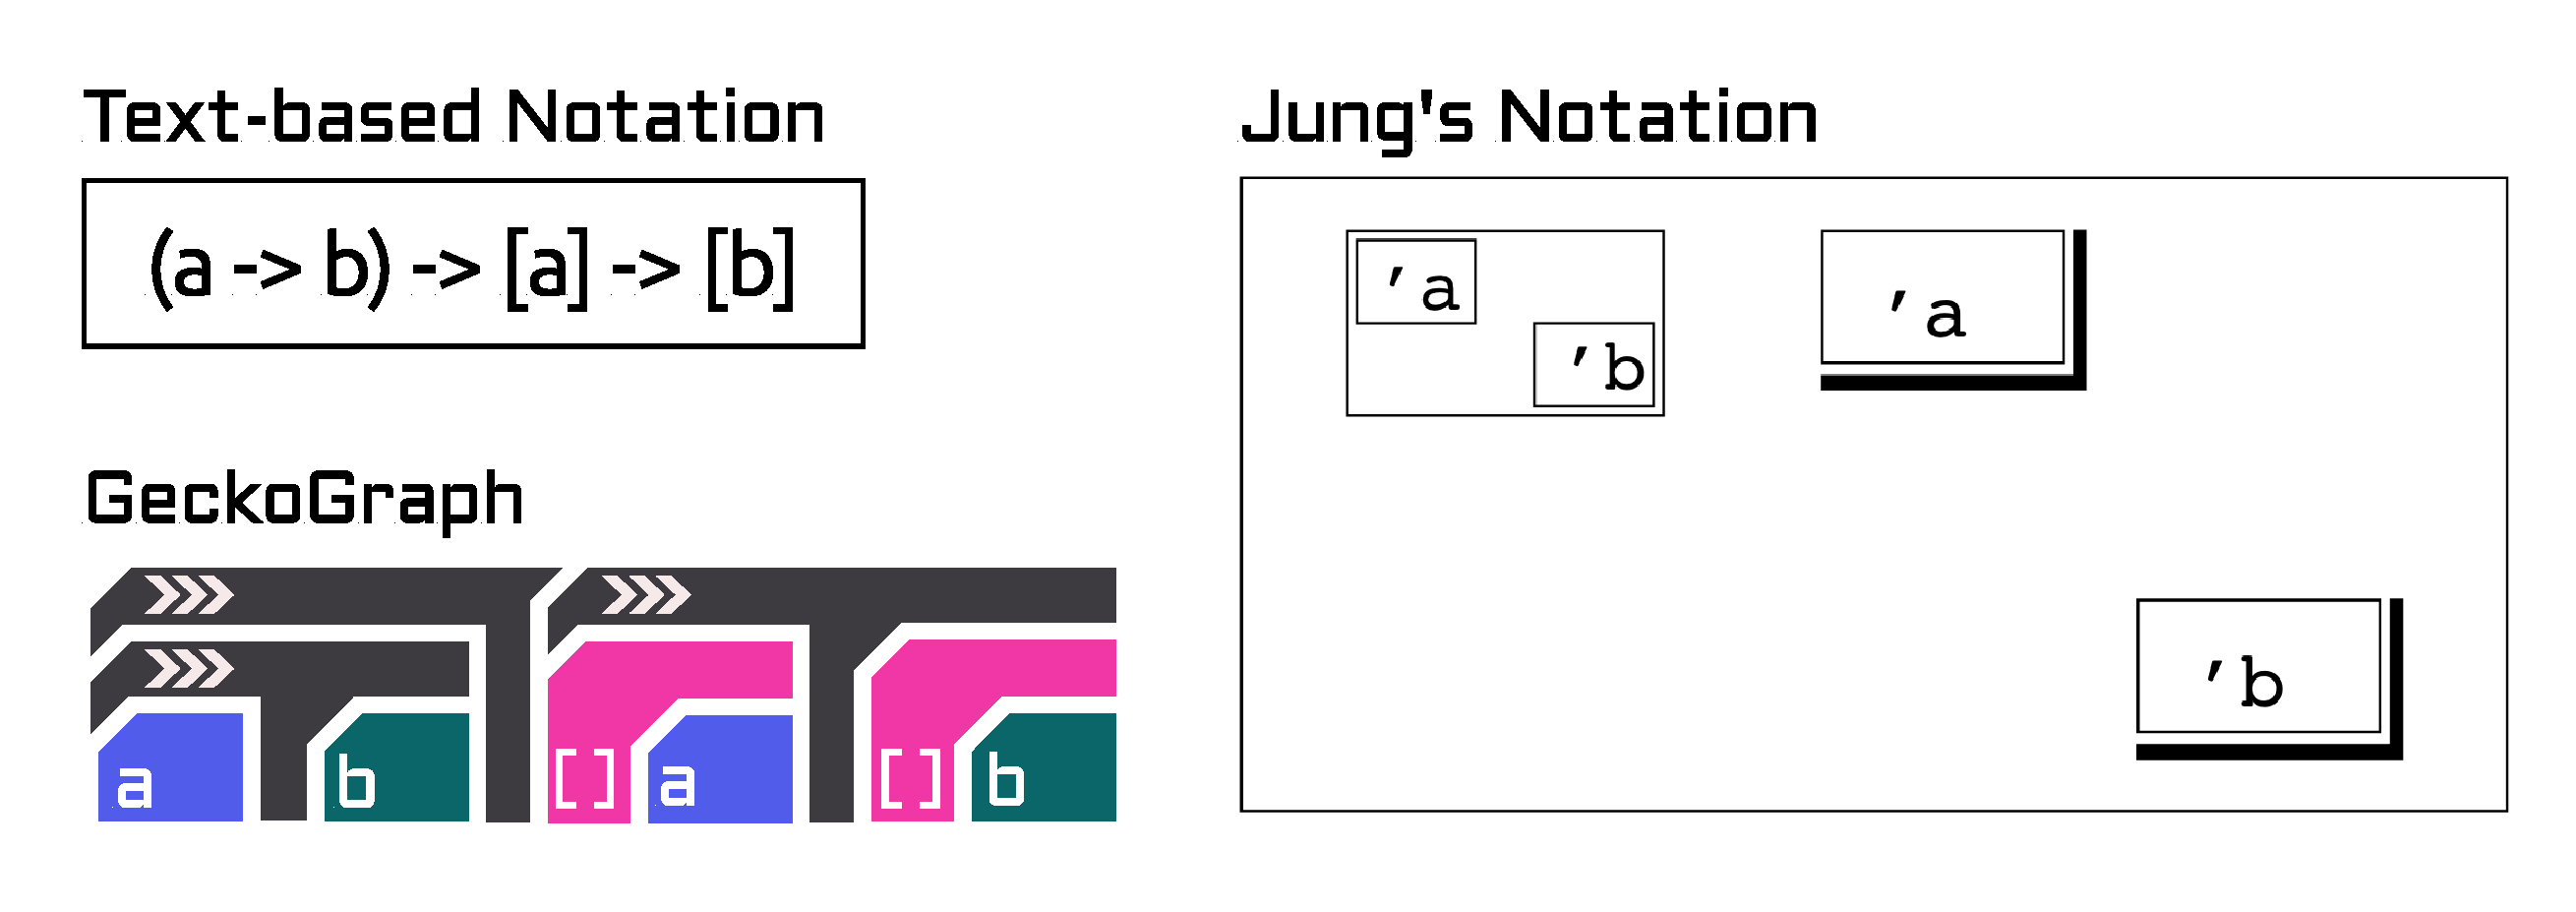
\includegraphics[width=\linewidth]{figures/Jung}
  \caption{
        \label{fig:jung}
        Comparison of the \texttt{map} function (\texttt{(a -> b) -> [a] -> [b]}) in text notation, GeckoGraph, and Jung’s notation.
  }
\end{figure}

More recent work, TYPEical~\cite{Moy2020-tr}, provides an interactive visualization of function types for exploring and comparing functions in R packages. 
This project is innovative in that it uses a Sankey diagram~\cite{Keiderling2012-ag} to illustrate the flow between collections of functions and the data types they operate on, as well as the frequency of their use, providing a high-level overview of the usage statistics. 
GeckoGraph shares TYPEical’s vision that visualization should support three key tasks: \textbf{finding functions}, \textbf{determining types}, and \textbf{comparing types}. 
However, unlike GeckoGraph, TYPEical’s visualization is generated ahead of time and is aimed primarily at language designers and core library developers rather than students or everyday programmers.

\begin{figure}
  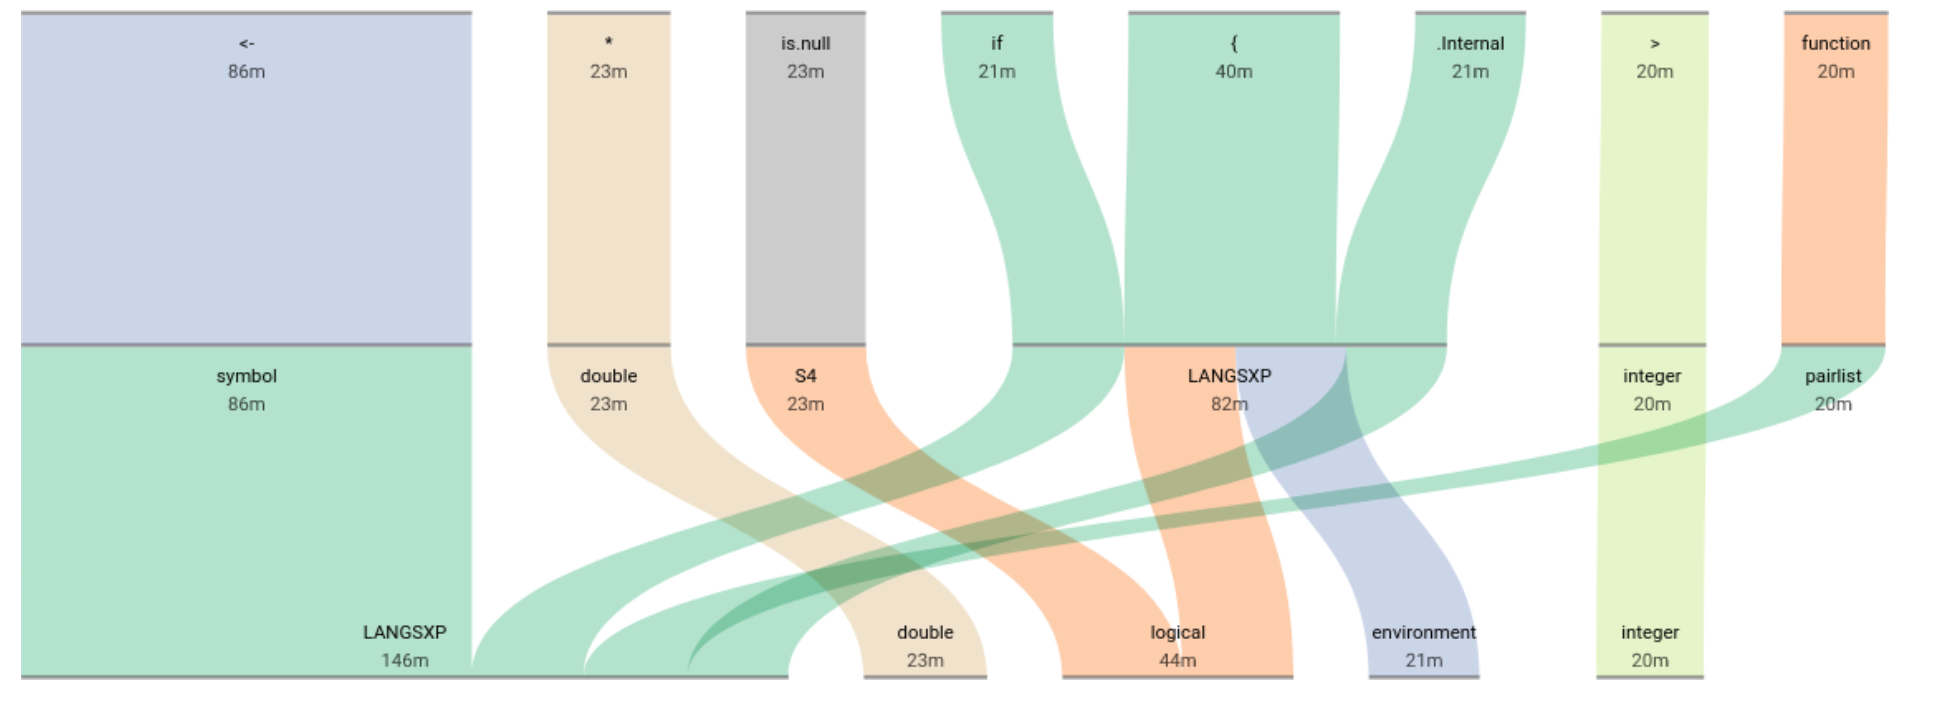
\includegraphics[width=\linewidth]{figures/Typical.png}
  \caption{
        \label{fig:typical}
        TYPEical’s type flow visualization. 
        The figure displays the type signatures of functions in R’s \texttt{base} library (top axis) and their first and second arguments (middle and bottom axes).
  }
\end{figure}

\subsection{Visualization in Programming}
\label{sec:viz-programming}

The use of visualization to improve the comprehension of polymorphic types is not new. 
It has been applied to represent document structures, runtime behavior, and static analysis results. 
For example, FluidEdt~\cite{Ou2015-vr} displays heap graphs in the editor margin, while I3~\cite{Beck2015-my} presents search similarity and change history through compact block-based diagrams. 
Almeida et~al.~\cite{Almeida2022-bv} introduced a visualization technique to aid understanding of ownership and borrowing in Rust. 
Although graphical representations of types remain a relatively narrow field, it has been explored in research such as Clerici et~al.~\cite{Clerici2013-ru}, who proposed a graph-based type inference system that visualizes unification states.

GeckoGraph positions itself similarly to these projects, using color, shapes, and icons to provide easily interpretable visual cues. 
However, GeckoGraph focuses specifically on type-level information—an area largely unexplored by previous work. 
In addition, GeckoGraph was evaluated through a larger and more diverse study, including participants with a broader range of programming experience.

\subsection{Visual vs. Textual Representation}
\label{sec:visual-vs-textual}

Many studies have compared visual programming environments with textual ones. 
Research~\cite{Noone2018-wl, Da_Silva_Ribeiro2014-tm, Cliburn2008-jo, Daly2011-is} consistently shows that students taught with visual programming languages demonstrate greater confidence, retention, and enjoyment compared to those using purely textual languages. 
While following a similar trend, GeckoGraph is designed as a complement to text-based notation rather than a replacement for it.

Several tools have explored the effect of visual augmentation—adding visual representations alongside textual code. 
For example, Greenfoot~\cite{Montero2010-uh} integrates visual and textual programming elements to support learning, while PILeT~\cite{Alshaigy2015-wy} adapts its presentation style to users’ preferences. 
Both systems report positive effects of visual augmentation. 
Although GeckoGraph also combines visual and textual representations, it differs in that prior studies focused on imperative languages such as Java and Python, whereas our evaluation investigates its effect in a functional programming context (Haskell).


\section{Conclusion and Future Work}
In this paper, we propose GeckoGraph, a graphical notation for type annotations in functional programming languages. GeckoGraph aims to complement traditional text-based type notation by making reading, understanding, and comparing types easier. We conducted a large-scale human study using GeckoGraph, comparing it to text-based type notation. This is the largest user study on functional programming we are aware of. Although no significant effect was found on the overall time to complete each programming task, we found a modest effect on the success rate in the beginner group. In one of the more difficult programming tasks, we find that GeckoGraph significantly improves the success rate by 14.5\% for beginners and 11.2\% for less experienced programmers.

Our work in this area opens many new directions for future research.  In particular:

\noindent\textbf{In-the-wild Studies}
Although our experiment scenarios are drawn from real-world programming tasks, a certain level of variable control is still applied to remove the effect of familiarity with the tools and libraries. However, it is necessary to assess the usefulness of tools such as GeckoGraph in terms of their real-life usage. Different research methods should be used to study the effects of GeckoGraph on realistic programming tasks. This may include field deployments or case studies. 

\noindent\textbf{Alternative Type Visualization}
We strongly believe that visualization is an underutilized technique in this effort. GeckoGraph focuses on a faithful view of the tree structure of programming types. However, many more areas and types demand a visual approach. For instance, visualizing the ordinal relationship of subsumption or visualizing the numeric values in dependently typed ``type programs". 

\bibliographystyle{elsarticle-num} 
\bibliography{paperpile}

\appendix
\section{User study tasks} \label{levels}
We provide all the level settings we used in our user study. The tasks are open source and available for evaluation\footnote{https://zerotohero.fly.dev}. However, this can be attempted locally with a Haskell interpreter or even with a pen and paper. The target type is the desired type signature for the function \texttt{zeroToHero}. The available functions show a list of functions that are allowed to be used in the implementation. It is not required to use all the available functions, and it is not forbidden to use any other functions or variables outside the provided functions; even the Haskell prelude is not available. 


\subsection{Level 1: Trial run}

\paragraph{Target Type } 
\begin{itemize}
    \item \texttt{zeroToHero :: Zero a -> Hero a}
\end{itemize}

\paragraph{Available Functions} 
\begin{itemize}
    \item \texttt{f :: Zero a -> Hero a}
\end{itemize}

\paragraph{Possible Solution} 
\begin{itemize}
    \item \texttt{zeroToHero z = f z}
\end{itemize}


\subsection{Level 2: Assembly required}

\paragraph{Target Type} 
\begin{itemize}
    \item \texttt{zeroToHero :: Zero a -> Hero a}
\end{itemize}

\paragraph{Available Functions} 
\begin{itemize}
    \item \texttt{runZero :: Zero a -> a}
    \item \texttt{mkHero :: a -> Hero a}
    \item \texttt{(\$) :: (a -> b) -> a -> b}
\end{itemize}

\paragraph{Possible Solution} 
\begin{itemize}
    \item \texttt{zeroToHero z = mkHero (runZero z)}
\end{itemize}

\subsection{Level 3: Which path?}
\paragraph{Target Type } 
\begin{itemize}
    \item \texttt{zeroToHero :: Zero a -> Hero (a, a)}
\end{itemize}

\paragraph{Available Functions} 
\begin{itemize}
    \item \texttt{f1 :: Zero a -> Hero a}
    \item \texttt{f2 :: Zero a -> (a, a)}
    \item \texttt{f3 :: Hero a -> Hero (a, a)}
    \item \texttt{(\$) :: (a -> b) -> a -> b}
    \item \texttt{(.) :: (b -> c) -> (a -> b) -> a -> c}
\end{itemize}

\paragraph{Possible Solution} 
\begin{itemize}
    \item \texttt{zeroToHero z = f3 . f1 \$ z}
\end{itemize}


\subsection{Level 4: A repeating pattern}
\paragraph{Target Type } 
\begin{itemize}
    \item \texttt{zeroToHero :: Zero a b -> Hero b b}
\end{itemize}

\paragraph{Available Functions} 
\begin{itemize}
    \item \texttt{f1 :: Zero a b -> Hero b a}
    \item \texttt{f2 :: Zero a a -> Hero a a}
    \item \texttt{f3 :: Zero a b -> Zero b a}
    \item \texttt{f4 :: Zero a b -> Zero b b}
    \item \texttt{(\$) :: (a -> b) -> a -> b}
    \item \texttt{(.) :: (b -> c) -> (a -> b) -> a -> c}
\end{itemize}

\paragraph{Possible Solution} 
\begin{itemize}
    \item \texttt{zeroToHero z = f2 . f4 \$ z}
\end{itemize}


\subsection{Level 5: A perfect pair}
\paragraph{Target Type } 
\begin{itemize}
    \item \texttt{zeroToHero :: Zero a b -> Hero b b}
\end{itemize}

\paragraph{Available Functions} 
\begin{itemize}
    \item \texttt{fst :: (a, b) -> a}
    \item \texttt{snd :: (a, b) -> b}
    \item \texttt{f1 :: Zero a b -> Hero b a}
    \item \texttt{f2 :: Zero a a -> Hero a a}
    \item \texttt{f3 :: Zero a b -> Zero b a}
    \item \texttt{f4 :: Zero a b -> Zero b b}
    \item \texttt{(\$) :: (a -> b) -> a -> b}
    \item \texttt{(.) :: (b -> c) -> (a -> b) -> a -> c}
\end{itemize}

\paragraph{Possible Solution} 
\begin{itemize}
    \item \texttt{zeroToHero z = snd .f3 . f1 \$ z}
\end{itemize}


\subsection{Level 6: Monty Hall}
\paragraph{Target Type } 
\begin{itemize}
    \item \texttt{zeroToHero :: Zero a b c -> Hero c a}
\end{itemize}

\paragraph{Available Functions} 
\begin{itemize}
    \item \texttt{f1 :: Zero a b c-> Zero c b a}
    \item \texttt{f2 :: Zero a b c -> Zero a c c}
    \item \texttt{f3 :: Zero a b c -> Hero b c}
    \item \texttt{(\$) :: (a -> b) -> a -> b}
    \item \texttt{(.) :: (b -> c) -> (a -> b) -> a -> c}
\end{itemize}

\paragraph{Possible Solution} 
\begin{itemize}
    \item \texttt{zeroToHero z = f3 . f1 . f2 \$ z}
\end{itemize}

\subsection{Level 7: TIE fighter}
\paragraph{Target Type } 
\begin{itemize}
    \item \texttt{zeroToHero :: Zero a b c -> Hero c}
\end{itemize}

\paragraph{Available Functions} 
\begin{itemize}
    \item \texttt{f1 :: Zero a b c -> Hero (a -> b)}
    \item \texttt{f2 :: Zero a b c -> Hero (b -> c)}
    \item \texttt{f3 :: Zero a b c -> Hero a}
    \item \texttt{(<\$>) :: (a -> b) -> Hero a -> Hero b}
    \item \texttt{(<*>) :: Hero (a -> c) -> Hero a -> Hero c}
    \item \texttt{(\$) :: (a -> b) -> a -> b}
    \item \texttt{(.) :: (b -> c) -> (a -> b) -> a -> c}
\end{itemize}

\paragraph{Possible Solution} 
\begin{itemize}
    \item \texttt{zeroToHero z = f2 z <*> (f1 z <*> f3 z)}
\end{itemize}

\subsection{Level 8: The middle man}
\paragraph{Target Type } 
\begin{itemize}
    \item \texttt{zeroToHero :: (a -> d) -> (b -> d) -> (c -> d) -> Zero a b c ->  Hero a d c}
\end{itemize}

\paragraph{Available Functions} 
\begin{itemize}
    \item \texttt{f1 :: Zero a b c -> Zero c a b}
    \item \texttt{f2 :: Zero a b c -> Hero a b c}
    \item \texttt{fmap :: (c -> d) -> Zero a b c -> Zero a b d}
    \item \texttt{(\$) :: (a -> b) -> a -> b}
    \item \texttt{(.) :: (b -> c) -> (a -> b) -> a -> c}
\end{itemize}

\paragraph{Possible Solution} 
\begin{itemize}
    \item \texttt{zeroToHero ad bd cd z = f2  . f1  . f1  . fmap bd  . f1 \$ z}
\end{itemize}

\subsection{Level 9: Split the difference}
\paragraph{Target Type } 
\begin{itemize}
    \item \texttt{zeroToHero :: Zero a b c d ->  Hero d d d d}
\end{itemize}

\paragraph{Available Functions} 
\begin{itemize}
    \item \texttt{f1 :: Zero a b c d -> Zero a a b b}
    \item \texttt{f2 :: Zero a b c d -> Hero c c d d}
    \item \texttt{f3 :: Zero a b c d -> Zero d c b a}
    \item \texttt{(\$) :: (a -> b) -> a -> b}
    \item \texttt{(.) :: (b -> c) -> (a -> b) -> a -> c}
\end{itemize}

\paragraph{Possible Solution} 
\begin{itemize}
    \item \texttt{zeroToHero ad bd cd z = f2 \$ f1 \$ f1 \$ f3 \$ z}
\end{itemize}


\subsection{Level 10: The roller coaster}
\paragraph{Target Type } 
\begin{itemize}
    \item \texttt{zeroToHero :: Zero (a -> b -> c -> d) a b c  -> Hero d}
\end{itemize}

\paragraph{Available Functions} 
\begin{itemize}
    \item \texttt{f1 :: Zero (a -> b) a c d -> Zero () b c d}
    \item \texttt{f2 :: Zero a b c d -> Zero b c d a}
    \item \texttt{f3 :: Zero a b c d -> Hero d}
    \item \texttt{(\$) :: (a -> b) -> a -> b}
    \item \texttt{(.) :: (b -> c) -> (a -> b) -> a -> c}
\end{itemize}

\paragraph{Possible Solution} 
\begin{itemize}
    \item \texttt{zeroToHero z = f3 . f2 . f2 . f1 . f2 . f1 . f2 . f1 \$ z}
\end{itemize}


\end{document}
\endinput
